\documentclass[sigconf,nonacm]{acmart}

%% Enable subfigures
\usepackage{subfigure}
%% Enable numbers in scientific format.
\usepackage{siunitx}
%% Enable enumerate start from.
\usepackage{enumitem}

%% Enable theorems
\newtheorem{theorem}{Theorem}[section]
\newtheorem{lemma}[theorem]{Lemma}

%% Enable algorithms
\usepackage{algorithm}
\usepackage[noend]{algpseudocode}
\let\ReturnInline\Return
\renewcommand{\Return}{\State\ReturnInline}
\algrenewcommand\algorithmicrequire{$\rhd$}
\algrenewcommand\algorithmicensure{$\square$}

%% Fonts used in the template cannot be substituted; margin 
%% adjustments are not allowed.
\AtBeginDocument{%
  \providecommand\BibTeX{{%
    \normalfont B\kern-0.5em{\scshape i\kern-0.25em b}\kern-0.8em\TeX}}}

%% Rights management information.
\setcopyright{acmcopyright}
\copyrightyear{2018}
\acmYear{2018}
\acmDOI{XXXXXXX.XXXXXXX}

%% These commands are for a PROCEEDINGS abstract or paper.
\acmConference[Conference acronym 'XX]{Make sure to enter the correct
  conference title from your rights confirmation emai}{June 03--05,
  2018}{Woodstock, NY}
%% Title of the proceedings is different from ``Proceedings of ...''?
% \acmBooktitle{Woodstock '18: ACM Symposium on Neural Gaze Detection,
%  June 03--05, 2018, Woodstock, NY} 
% \acmPrice{15.00}
% \acmISBN{978-1-4503-XXXX-X/18/06}

%% Submission ID.
% \acmSubmissionID{123-A56-BU3}

%% Use the "author year" style of citations and references?
% \citestyle{acmauthoryear}

%% Message
\newcommand{\kk}[1]{{{\color{red} #1}}}
\newcommand{\ds}[1]{{{\color{blue} #1}}}
\newcommand{\su}[1]{{{\color{green} #1}}}

%% Ignore block
\newcommand{\ignore}[1]{}
%% Mark block as done
\newcommand{\ok}[1]{}




\begin{document}

%% Full title of the paper.
\title[A Fast Parallel Approach for Neighborhood-based Link Prediction by Disregarding Large Hubs]{A Fast Parallel Approach for Neighborhood-based \\Link Prediction by Disregarding Large Hubs}

%% Short title to be used in page headers (optional).
% \title[short title]{full title}
% \subtitle{Something other than the title}

%% Authors and their affiliations.
\author{Subhajit Sahu}
\email{subhajit.sahu@research.iiit.ac.in}
\affiliation{%
  \institution{IIIT Hyderabad}
  \streetaddress{Professor CR Rao Rd, Gachibowli}
  \city{Hyderabad}
  \state{Telangana}
  \country{India}
  \postcode{500032}
}

%% Concise author list in page headers.
%\renewcommand{\shortauthors}{Sahu, Kothapalli, and Banerjee, et al.}

%% Show page numbers.
\settopmatter{printfolios=true}

%% Short summary of the work to be presented in the article.
\begin{abstract}
Link prediction can help rectify inaccuracies in various graph algorithms, stemming from unaccounted-for or overlooked links within networks. However, many existing works use a baseline approach, which incurs unnecessary computational costs due to its high time complexity. Further, many studies focus on smaller graphs, which can lead to misleading conclusions. Here, we study the prediction of links using neighborhood-based similarity measures on large graphs. In particular, we improve upon the baseline approach (IBase), and propose a heuristic approach that additionally disregards large hubs (DLH), based on the idea that high-degree nodes contribute little similarity among their neighbors. On a server equipped with dual 16-core Intel Xeon Gold 6226R processors, DLH is on average $1019\times$ faster than IBase, especially on web graphs and social networks, while maintaining similar prediction accuracy. Notably, DLH achieves a link prediction rate of $38.1M$ edges/s and improves performance by\ignore{at a rate of} $1.6\times$ for every doubling of threads.
\end{abstract}

% Link prediction aims to anticipate missing or future connections in a network using known interactions and structure, often employing similarity measures for their simplicity and computational efficiency. While many studies focus on smaller graphs, this report addresses the evaluation of algorithms on larger networks and introduces a heuristic for efficient computation. Additionally, the commonly used baseline approach, despite its simplicity, incurs unnecessary computational costs due to its high time complexity.

%% The code below is generated by the tool at http://dl.acm.org/ccs.cfm.
\begin{CCSXML}
<ccs2012>
<concept>
<concept_id>10003752.10003809.10010170</concept_id>
<concept_desc>Theory of computation~Parallel algorithms</concept_desc>
<concept_significance>500</concept_significance>
</concept>
<concept>
<concept_id>10003752.10003809.10003635</concept_id>
<concept_desc>Theory of computation~Graph algorithms analysis</concept_desc>
<concept_significance>500</concept_significance>
</concept>
</ccs2012>
\end{CCSXML}

% \ccsdesc[500]{Theory of computation~Parallel algorithms}
% \ccsdesc[500]{Theory of computation~Graph algorithms analysis}

%% Pick words that accurately describe the work being presented.
\keywords{Parallel Link prediction, Local/Neighborhood-based}

% \received{20 February 2007}
% \received[revised]{12 March 2009}
% \received[accepted]{5 June 2009}



%% Process the author and title information.
\maketitle

\section{Introduction}
\label{sec:introduction}
Most real world networks are incomplete \cite{kim2011network, wang2014link}. These networks lie somewhere in the range of a deterministic and a purely random structure, and are thus partially predictable \cite{lu2015toward}. Link prediction is the problem of identifying potentially missing/undiscovered connections in such networks \cite{marchette2008predicting, kim2011network}, or even forecasting future connections \cite{bringmann2010learning, juszczyszyn2011link}, by examining the current network structure\ignore{\cite{zhou2021progresses}}. This is useful in various applications, such as recommending items for online purchase \cite{akcora2011network}, helping people to find potential collaborators \cite{mori2012machine, tang2012cross},\ignore{predicting co-authorships in academic research networks \cite{pavlov2007finding, wohlfarth2008semantic}, identifying abnormal communications \cite{huang2009time}} assessing trustworthiness of individuals \cite{alnumay2019trust}, uncovering criminal activities and individuals \cite{berlusconi2016link, lim2019hidden}\ignore{, detecting anomalies \cite{huang2006link}}, and predicting new protein-protein interactions or generating hypotheses \cite{cannistraci2013link, nasiri2021novel}.

Similarity measures are frequently employed to predict the likelihood of missing or future links between unconnected nodes in a network \cite{wang2014link, arrar2023comprehensive}. The principle is straightforward: higher similarity indicates a greater likelihood of connection \cite{wang2014link}. The choice of metric depends on the network's characteristics, with no single metric dominating across different datasets \cite{arrar2023comprehensive, zhou2021progresses}. Local / neighborhood-based similarity metrics such as Common Neighbors, Jaccard Coefficient,  S{\o}rensen Index, Salton Cosine similarity, Hub Promoted, Hub Depressed, Leicht-Holme-Nerman, Adamic-Adar, and Resource Allocation, which are based of are based on neighborhood information within a path distance of two, remain popular \cite{arrar2023comprehensive, wang2014link}. This is due to their simplicity, interpretability \cite{pai2019netdx, barbieri2014follow}, computational efficiency \cite{garcia2014link}, and the ability to capture underlying structural patterns.\ignore{Further, they are often combined with other metrics.}

However, early studies often evaluate a limited number of algorithms on small networks --- this can result in misleading conclusions \cite{zhou2021progresses, zhou2021experimental}. Further, much existing research does not address link prediction for large networks with close to a billion edges \cite{muscoloni2022adaptive, mumin2022efficient, nasiri2021novel, xian2021towards, ghasemian2020stacking, mara2020benchmarking, wang2019link, xu2019distributed, mohan2017scalable, cui2016bounded, garcia2014link, papadimitriou2012fast}. As the collection of data, represented as graphs, reach unprecedented levels, it becomes necessary to design efficient parallel algorithms for link prediction on such graphs. While link prediction algorithms are often pleasingly parallel, most studies do not address the design of suitable data structures for efficient computation of scores.

Further, the link prediction problem faces significant imbalance, with the number of known present links often several order of magnitude less than known absent links. This imbalance hinders the effectiveness of many link prediction methods, particularly on large networks \cite{wang2014link, garcia2014link}. Thus, heuristics are needed to minimize the computation needed, without sacrificing on quality.\ignore{To assess the accuracy of link prediction algorithms, observed links $E$ are split into a training set $E^T$ and a probe set $E^P$ for evaluation.} Quality assessment measures for link prediction include precision, recall, F1 score, accuracy, and Area Under the Receiver Curve (AUC). While AUC is commonly used \cite{arrar2023comprehensive}, it may provide misleading results\ignore{, by giving high scores to algorithms that successfully rank many negatives in the bottom} \cite{yang2015evaluating, lichtnwalter2012link}, leading to our focus on F1 score.

\ignore{How do you explore the neighbors of each node, and compute intersection? What is a super naive way to do the above?}




\subsection{Our Contributions}

This technical report proposes an approach for significantly improving the performance of existing local/neighbor-based link prediction techniques, both in terms of runtime and precision.

GVE-Leiden\footnote{https://github.com/puzzlef/neighborhood-link-prediction-openmp}, an optimized parallel implementation of the Leiden algorithm for community detection on shared memory multicores. On a machine with two 16-core Intel Xeon Gold 6226R processors, GVE-Leiden achieves a processing rate of $352 M$ edges/s on a $3.8 B$ edge graph, and outperforms the original Leiden implementation, igraph Leiden, and NetworKit Leiden by $373\times$, $86\times$, and $7.2\times$ respectively, while identifying communities of the same quality as the first two implementations, and $26\%$ higher quality than NetworKit. Compared to GVE-Louvain, our parallel Louvain implementation, GVE-Leiden achieves an $11$-fold reduction in internally-disconnected communities, with only a $36\%$ increase in computation time. With doubling of threads, GVE-Leiden exhibits an average performance scaling of $1.6\times$.\ignore{This makes GVE-Leiden an attractive choice for high-quality community detection on massive graphs.}

In this poster, we parallelize link prediction and present algorithmic techniques to significantly accelerate it. In addition, we use the parallel Dynamic Frontier Hybrid Louvain-LPA algorithm for community detection to further accelerate the dynamic community detection algorithm.




%% - Use --- for a dash.
%% - Use ``camera-ready'' for quotes.
%% - Use {\itshape very} or \textit{very} for italicized text.
%% - Use \verb|acmart| or {\verb|acmart|} for mono-spaced text.
%% - Use \url{https://capitalizemytitle.com/} for URLs.
%% - Use {\bfseries Do not modify this document.} for important boldface details.
%% - Use \ref{fig:name} for referencing.

%% For a block of pre-formatted text: 
% \begin{verbatim}
%   \renewcommand{\shortauthors}{McCartney, et al.}
% \end{verbatim}

%% For a list of items:
% \begin{itemize}
% \item the ``ACM Reference Format'' text on the first page.
% \item the ``rights management'' text on the first page.
% \item the conference information in the page header(s).
% \end{itemize}

%% For a table:
% \begin{table}
%   \caption{Frequency of Special Characters}
%   \label{tab:freq}
%   \begin{tabular}{ccl}
%     \toprule
%     Non-English or Math&Frequency&Comments\\
%     \midrule
%     \O & 1 in 1,000& For Swedish names\\
%     $\pi$ & 1 in 5& Common in math\\
%     \$ & 4 in 5 & Used in business\\
%     $\Psi^2_1$ & 1 in 40,000& Unexplained usage\\
%   \bottomrule
% \end{tabular}
% \end{table}

%% For a full-width table:
% \begin{table*}
%   \caption{Some Typical Commands}
%   \label{tab:commands}
%   \begin{tabular}{ccl}
%     \toprule
%     Command &A Number & Comments\\
%     \midrule
%     \texttt{{\char'134}author} & 100& Author \\
%     \texttt{{\char'134}table}& 300 & For tables\\
%     \texttt{{\char'134}table*}& 400& For wider tables\\
%     \bottomrule
%   \end{tabular}
% \end{table*}


%% For inline math:
% \begin{math}
%   \lim_{n\rightarrow \infty}x=0
% \end{math},

%% For a numbered equation:
% \begin{equation}
%   \lim_{n\rightarrow \infty}x=0
% \end{equation}

%% For an unnumbered equation:
% \begin{displaymath}
%   \sum_{i=0}^{\infty} x + 1
% \end{displaymath}

%% For a figure:
% \begin{figure}[h]
%   \centering
%   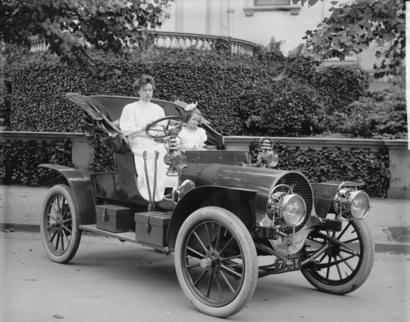
\includegraphics[width=\linewidth]{inc/sample-franklin}
%   \caption{1907 Franklin Model D roadster. Photograph by Harris \&
%     Ewing, Inc. [Public domain], via Wikimedia
%     Commons. (\url{https://goo.gl/VLCRBB}).}
%   \Description{A woman and a girl in white dresses sit in an open car.}
% \end{figure}

%% For a teaser figure.
% \begin{teaserfigure}
%   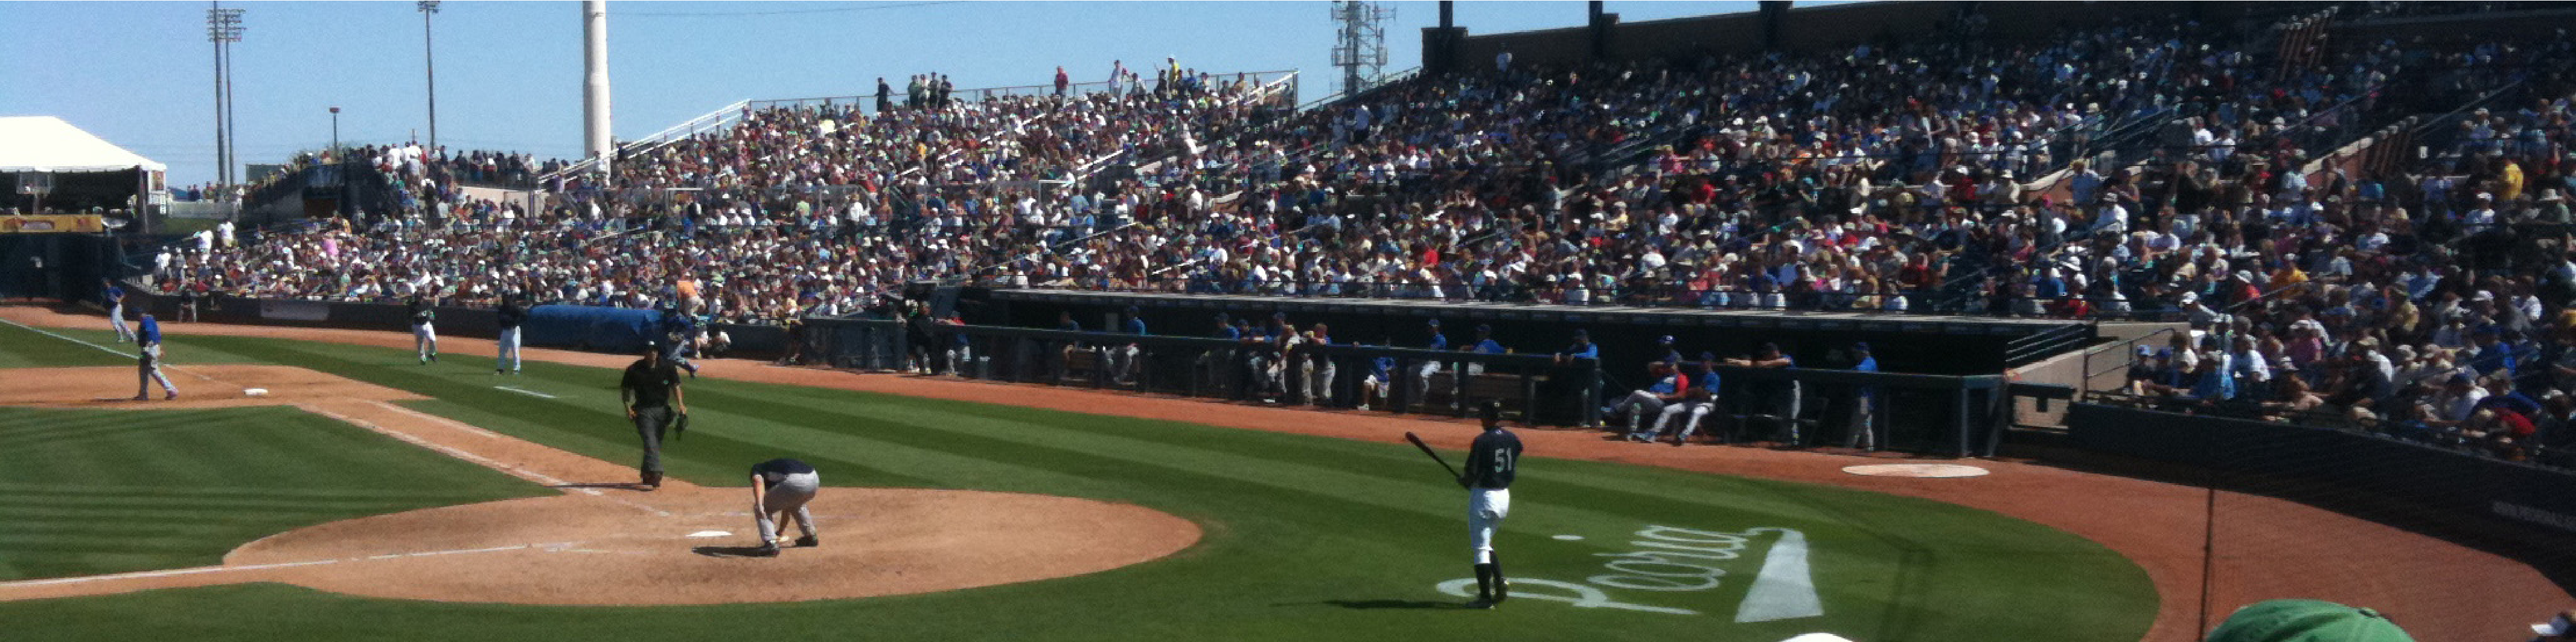
\includegraphics[width=\textwidth]{sampleteaser}
%   \caption{figure caption}
%   \Description{figure description}
% \end{teaserfigure}


\section{Related work}
\label{sec:related}
Link prediction in network analysis involves diverse algorithms. This include the use of similarity-based methods, dimensionality reduction, and machine learning \cite{arrar2023comprehensive}. As mentioned earlier, the use of similarity measures for link prediction is based on the intuition that the more similar a pair of nodes are, the more likely a link between them, and vice versa. This is consistent with the fact that users tend to create relationships with people who are similar in education, religions, interests and locations \cite{wang2014link}. Similarity measures are commonly classified into three categories: local, quasi-local, and global measures. Local measures calculate scores based on the neighborhood information of nodes with a path distance less than two; global measures use information from the entire network to calculate scores with a path distance greater than two; while quasi-local measures combine local and global measures and calculate scores for nodes with a path distance of no more than two. Other similarity based approaches include the use of random walks and community detection \cite{arrar2023comprehensive}.

Dimensionality reduction techniques \cite{coskun2015link} attempt to map the network's information into a lower dimensional space, while preserving its structural information and components. These include embedding-based methods and matrix factorization based methods. On the other hand, machine learning techniques utilize relevant extracted features from the network data to predict the probability of a link forming between two nodes based on these features. These include the use of supervised \cite{kumari2022supervised, abuoda2020link, lichtenwalter2010new}, unsupervised \cite{rossi2021closing}, reinforcement, and deep learning \cite{cui2018survey, arrar2023comprehensive}.

While the above techniques effectively capture nonlinear relationships between nodes, and enable more accurate predictions within complex networks than similarity based approaches, they come with certain drawbacks. Embedding-based methods face challenges in predicting links for nodes with high centrality --- which have complex connectivity patterns and numerous connections to other nodes \cite{arrar2023comprehensive}. Matrix factorization methods depend heavily on accurately representing the observed network through a low-rank matrix, which may not be feasible for networks with complex structures \cite{martinez2016survey, arrar2023comprehensive}. Further, they require significant computational resources and may result in overfitting if it is not regulated properly, particularly in large-scale networks \cite{arrar2023comprehensive}.

Machine learning based approaches have their own set of drawbacks. Supervised learning based methods require high-quality features to be extracted from the network, which requires domain expertise and can be challenging. As the network evolves, these features may also get outdated. They also need a large labelled dataset, obtaining which can be a time consuming task. Finally, supervised learning techniques have a high time complexity. While deep learning does not require feature extraction, it still requires a substantial about of labelled data, which can be challenging to acquire. Further, the interpretability of deep learning models is limited, and overfitting is also a potential concern.

Similarity-based link prediction methods continue to stay relevant, despite their usually lower prediction accuracy. This is because the size of graphs originated from the web, social networks or biological relations force us to use very simple algorithms if those graphs are to be computed in acceptable time \cite{garcia2014link}. Similarity-based link prediction methods are highly cost-effective, as they offer competitive prediction quality with their low complexity in time and space \cite{zhou2021progresses}. Further, in certain applications like friend recommendation, preference is given to predictions with explanations, a feature not readily achievable through machine learning based techniques \cite{barbieri2014follow}.

%% ON COMMON NEIGHBORS
Yang et al. \cite{yang2015new} introduce the Local Neighbors Link (LNL) measure, motivated by cohesion between common neighbors and predicted nodes, and implemented it on both MapReduce and Spark. Cui et al. \cite{cui2016bounded} present a parallel algorithm for efficiently evaluating Common Neighbors (CN) similarity, obtaining node pairs with CN values surpassing a specified lower bound. Guo et al. \cite{guo2019node} propose Common Neighbour Tightness (CNT), incorporating the aggregation degree of common neighbors by considering their proximity through local information and neighborhood tightness. Rafiee et al. \cite{rafiee2020cndp} introduce Common Neighbors Degree Penalization (CNDP), which factors in clustering coefficient as a structural property and considers neighbors of shared neighbors. Mumin et al. \cite{mumin2022efficient} contribute an algorithm combining common neighbors and node degree distribution to estimate link presence likelihood between two nodes based on local information.

%% ON RANDOM WALK, DIFFUSION
Papadimitriou et al. \cite{papadimitriou2012fast} introduce a similarity-based algorithm employing traversals on paths of limited length, grounded in the small world hypothesis. Their approach extends to directed and signed graphs, with discussions on a potential MapReduce implementation. Kalkan and Hambiralovic \cite{kalkanfinding} propose link prediction based on Personalized PageRank. Vega-Oliveros et al. \cite{vega2021link} investigate the use of susceptible-infected-recovered and independent cascade diffusion models. Their progressive-diffusion (PD) method, founded on nodes' propagation dynamics, provides a stochastic discrete-time rumor model for link prediction.

%% ON COMMUNITY
Mohan et al. \cite{mohan2017scalable} introduce a hybrid similarity measure utilizing parallel label propagation for community detection and a parallel community information-based Adamic-Adar measure, employing the Bulk Synchronous Parallel (BSP) programming model. Wang et al. \cite{wang2019link} propose a link prediction algorithm incorporating an adjustable parameter based on community information (CI), applying it to various similarity indices and a family of CI-based indices. They also develop a parallel algorithm for large-scale complex networks using Spark GraphX. Bastami et al. \cite{bastami2019gravitation} present a gravitation-based link prediction approach, enhancing local and global predictions through the integration of node features, community information, and graph properties. Saifi et al. \cite{saifi2023fast} propose an approach that accelerates link prediction using local and path-based similarity measures by operating on the connected components of a network rather than the entire network.

%% ON APPROXIMATION
Shin et al. \cite{shin2012multi} introduce Multi-Scale Link Prediction (MSLP), employing a tree-structured approximation algorithm for efficient link prediction in large networks. Garcia-Gasulla and Cort{\'e}s \cite{garcia2014link} propose a local link prediction algorithm based on an underlying hierarchical model, emphasizing aspects of parallelization, approximation, and data locality for computational efficiency. Ferreira et al. \cite{ferreira2019scalability} present a multilevel optimization paradigm to enhance the scalability of any link prediction algorithm by reducing the original network to a coarsened version. Benhidour et al. \cite{benhidour2022approach} propose a link prediction method for directed networks, leveraging the similarity-popularity paradigm. The algorithms approximate hidden similarities as shortest path distances, using edge weights that capture and factor out links' asymmetry and nodes' popularity.

%% ON BIPARTITE
\ignore{Aslan and Kaya \cite{aslan2018topic} introduce a similarity-based method using weighted projection to predict potential links between authors and topics in a large-scale bipartite academic information network. Sarhangnia et al. \cite{sarhangnia2022novel} present a similarity measure for link prediction in bipartite social networks, focusing on the neighborhood structure. Shifting to multiplex networks, Sharma and Singh \cite{sharma2016efficient} propose an algorithm for weight prediction using link similarity measures, contributing to the efficient analysis of multiplex network structures. ORCS.}

As mentioned earlier, similarity-based algorithms are competitive to other high-quality dimensionality reduction and machine learning techniques, thanks to their simplicity, interpretability \cite{pai2019netdx, barbieri2014follow}, and computational efficiency \cite{garcia2014link} --- and are thus often combined with other techniques \cite{kumari2022supervised, abuoda2020link, pai2019netdx}. However, the evaluation of these algorithms on large networks is crucial, as testing on small networks can yield misleading conclusions \cite{zhou2021progresses, zhou2021experimental}. Despite this, a significant portion of the discussed works focuses on small \cite{guo2019node, rafiee2020cndp, mumin2022efficient, papadimitriou2012fast, vega2021link, saifi2023fast, ferreira2019scalability, benhidour2022approach} to medium-scale graphs \cite{yang2015new, cui2016bounded, kalkanfinding, mohan2017scalable, wang2019link, bastami2019gravitation, shin2012multi, garcia2014link}, with less than a million or billion edges. Parallelism becomes essential on large networks, and while some approaches, such as the ones based on common neighbors \cite{yang2015new, cui2016bounded}, random walks \cite{papadimitriou2012fast}, community structures \cite{mohan2017scalable, wang2019link}, and approximation \cite{garcia2014link}, incorporate parallelism, the design of suitable data structures for efficient score computation remains an often-overlooked aspect. This technical report aims to bridge both gaps, while also proposing a heuristic for efficient computation.


\section{Preliminaries}
\label{sec:preliminaries}
In an undirected graph $G(V, E)$ with sets of vertices $V$ and edges $E$, link prediction aims to identify missing or future edges from the set $U - E$, where $U$ contains all possible $|V|(|V|-1)/2$ edges in the graph \cite{zhou2021progresses}. Link prediction, thus, is akin to finding a needle in a haystack, as the correct edges need to be identified within a vast set of incorrect ones \cite{garcia2014link, wang2014link}. Garcia et. al \cite{garcia2014link} observe that this ratio goes from $1:11k$ in their best case to $1:27M$ in the worst case. Further, larger graphs more likely to be incomplete. These challenges make the study of link prediction crucial.

Link prediction often relies on similarity metrics between node pairs, reflecting the likelihood of missing or future links \cite{wang2014link, arrar2023comprehensive}. The idea is grounded in the tendency for users to connect with similar individuals. More similarity thus suggests a higher probability of a future link. A ranked list of potential links based on similarity scores can then be used to predict the top-$k$ links are most likely to appear (on were missing) \cite{wang2014link}. Similarity measures are commonly categorized into local, quasi-local, and global measures. Local / neighborhood-based metrics, like Common Neighbours (CN), are calculated based on neighborhood information within a path distance of two. Global indices use network-wide information, while quasi-local indices combine both for distances up to two \cite{arrar2023comprehensive}.

As brought up earlier, despite typically having lower prediction accuracy than machine learning based approaches, similarity-based link prediction methods remain relevant due to the need for simple algorithms in handling large graphs \cite{garcia2014link}. Further, they are highly cost-effective, interpretable, and offer competitive prediction quality with low time and space complexity \cite{zhou2021progresses, barbieri2014follow}.




\subsection{Neighborhood-based Similarity Metrics}

We now discuss nine commonly used local / neighborhood-based similarity metrics for link prediction.


\subsubsection{Common Neighbors (CN)}

This metric, shown in Equation \ref{eq:cn}, counts the shared neighbors between two vertices, $a$ and $b$, in a graph \cite{newman2001clustering}. However, its lack of normalization may pose challenges when comparing node pairs with different degrees of connectivity.

\begin{equation}
\label{eq:cn}
  CN(a, b) = |\Gamma_a \cap \Gamma_b|
\end{equation}


\subsubsection{Jaccard Coefficient (JC)}

The Jaccard Coefficient (JC) \cite{jaccard1901etude} is a popular similarity measure\ignore{in network analysis and link prediction}. It offers a normalized assessment of similarity between nodes based on their neighborhoods. Defined by Equation \ref{eq:jc}, JC assigns higher values to node pairs with a greater proportion of common neighbors relative to their total neighbors.

\begin{equation}
\label{eq:jc}
  JC(a, b) = \frac{|\Gamma_a \cap \Gamma_b|}{|\Gamma_a \cup \Gamma_b|}
\end{equation}


\subsubsection{S{\o}rensen Index (SI)}

S{\o}rensen Index (SI) \cite{sorensen1948method}, also known as S{\o}rensen–Dice coefficient, is another similarity metric commonly applied in network analysis and link prediction. This metric, defined by Equation \ref{eq:si}, extends beyond solely accounting for the size of common neighbors and introduces the idea that nodes with lower degrees are more likely to form links.

\begin{equation}
\label{eq:si}
  SI(a, b) = \frac{|\Gamma_a \cap \Gamma_b|}{|\Gamma_a| + |\Gamma_b|}
\end{equation}


\subsubsection{Salton Cosine similarity (SC)}

The Salton Cosine similarity (SC) \cite{salton1973specification} essentially measures the cosine of the angle between the vectors representing the neighborhoods of nodes $a$ and $b$, as given in Equation \ref{eq:sc}. Similar to other metrics, a higher SC value indicates a greater similarity in the neighborhood structures of the nodes, implying a higher likelihood of a link between them.

\begin{equation}
\label{eq:sc}
  SC(a, b) = \frac{|\Gamma_a \cap \Gamma_b|}{\sqrt{|\Gamma_a| \cdot |\Gamma_b|}}
\end{equation}


\subsubsection{Hub Promoted (HP)}

The HP \cite{liben2003link} metric, defined by Equation \ref{eq:hp}, assesses topological overlap between two nodes in a graph. It is particularly influenced by the lower degree of nodes, and can be valuable in scenarios where the involvement of lower-degree nodes is considered important in understanding network connectivity.

\begin{equation}
\label{eq:hp}
  HP(a, b) = \frac{|\Gamma_a \cap \Gamma_b|}{min(|\Gamma_a|, |\Gamma_b|)}
\end{equation}


\subsubsection{Hub Depressed (HD)}

In contrast to the HP metric, the Hub Depressed (HD) score \cite{zhou2009predicting} is determined by the higher degrees of nodes, as illustrated by Equation \ref{eq:hd}. It can be particularly useful in cases where the influence of highly connected nodes on network structure is of interest.

\begin{equation}
\label{eq:hd}
  HD(a, b) = \frac{|\Gamma_a \cap \Gamma_b|}{max(|\Gamma_a|, |\Gamma_b|)}
\end{equation}


\subsubsection{Leicht-Holme-Nerman (LHN)}

The Leicht-Holme-Nerman (LHN) score \cite{leicht2006vertex} is a similarity metric that assigns high similarity to node pairs that exhibit a greater number of common neighbors than would be expected by random chance. One may use Equation \ref{eq:lhn} to compute the LHN score between two nodes $a$ and $b$ in a graph.

\begin{equation}
\label{eq:lhn}
  LHN(a, b) = \frac{|\Gamma_a \cap \Gamma_b|}{|\Gamma_a| \cdot |\Gamma_b|}
\end{equation}


\subsubsection{Adamic-Adar coefficient (AA)}

AA \cite{adamic2003friends} is a popular measure designed to capture the notion that connections to common neighbors with fewer links are more informative and indicative of similarity between nodes in a network. The formula in Equation \ref{eq:aa} assigns weights inversely proportional to the logarithm of the number of neighbors, reducing sensitivity to highly connected nodes.\ignore{AA highlights that links to less common neighbors provide more discriminative information about node similarity.}

\begin{equation}
\label{eq:aa}
  AA(a, b) = \sum_{c\ \in\ \Gamma_a \cup \Gamma_b} \frac{1}{\log{|\Gamma_c|}}
\end{equation}


\subsubsection{Resource Allocation (RA)}

The RA metric \cite{zhou2010solving} is based on the concept of heat diffusion in a network, emphasizing that heavily connected nodes may not play a critical role in facilitating resource flow between other nodes. Unlike AA, RA penalizes high-degree common neighbors more heavily. The score between nodes $a$ and $b$ is determined by Equation \ref{eq:ra}.

\begin{equation}
\label{eq:ra}
  RA(a, b) = \sum_{c\ \in\ \Gamma_a \cup \Gamma_b} \frac{1}{|\Gamma_c|}
\end{equation}

Note that the CN, AA, and RA metrics lack normalization, and thus only convey ranking information \cite{wang2014link}. In practical applications, one should choose the right metric based on the network's characteristics --- there is no universally dominating metric \cite{zhou2021progresses, ghasemian2020stacking, wang2014link, liben2003link}.




\subsection{Measuring Prediction Quality}

A number of measures are used to assess link prediction performance. These include precision, recall, F1 score, and Area Under the Receiver Curve (AUC) \cite{arrar2023comprehensive}. However, AUC is insufficient for early quality assessment, as it may inaccurately favor algorithms ranking many negatives at the bottom \cite{zhou2021progresses, yang2015evaluating, lichtnwalter2012link}. Accordingly, we focus on precision, recall, and F1 score in this report.


\subsubsection{Precision}

Precision measures the ratio of correctly predicted links $P^\checkmark$ to all predicted links $P = P^\checkmark \cup P^\times$, where $P^\times$ is the set of incorrectly predicted links \cite{arrar2023comprehensive, zhou2021progresses}. Equation \ref{eq:precision} provides the formula for precision computation.

\begin{equation}
\label{eq:precision}
  \text{Precision} = \frac{|P^\checkmark|}{|P|}
\end{equation}


\subsubsection{Recall}

Unlike precision, recall measures the ratio of correctly predicted links $P^\checkmark$ to the new ground-truth links $E^U$, as presented in Equation \ref{eq:recall} \cite{arrar2023comprehensive, zhou2021progresses}. If the number of predicted links is equal to the number of new ground-truth links, then recall is the same as precision \cite{zhou2021progresses, lu2011link, liben2003link}.

\begin{equation}
\label{eq:recall}
  \text{Recall} = \frac{|P^\checkmark|}{|E^U|}
\end{equation}


\subsubsection{F1 Score}

F1 score is a measure of the balance between precision and recall \cite{arrar2023comprehensive}. It is calculated as the harmonic mean of precision and recall, as shown in Equation \ref{eq:f1score}.

\begin{equation}
\label{eq:f1score}
  \text{F1 score} = 2 * \frac{\text{Precision} * \text{Recall}}{\text{Precision} + \text{Recall}}
\end{equation}

A majority of link prediction studies apply random division of the ground-truth edges $E$, into sets of observed $E^O$ and unobserved edges $E^U$ to assess link prediction performance \cite{zhou2021progresses}. The number of unobserved edges $|E^U|$ is commonly set at $10\%$ of total links in $E$, based on empirical findings that it yields statistically solid results without significantly altering the network's structure \cite{lu2015toward}.




\subsection{Baseline Approach for Neighborhood-based Link Prediction}

A baseline approach for neighborhood-based link prediction involves computing similarity scores between all non-connected node pairs $\{(i, j)\ |\ i, j \in V; (i, j) \notin E\}$, and returning the node pairs with top-$k$ scores as the predicted links. The similarity score is computed by assessing the commonality of neighbors between the two nodes. This approach is used by an number of studies previously mentioned \cite{gatadi2023lpcd, saifi2023fast, benhidour2022approach, mumin2022efficient, rafiee2020cndp, guo2019node, yang2015new, papadimitriou2012fast, wang2019link}. Notably, popular network analysis software packages such as NetworKit \cite{staudt2016networkit} and igraph \cite{csardi2006igraph} also implement this baseline approach.

While this approach is simple to understand, it has severe computational costs. Finding the common neighbors $\Gamma_i \cap \Gamma_j$ of node pairs $(i, j)$ using a naive method has a time complexity of $O(D^2)$, where $D$ is the degree of the maximum degree node in the graph. This results in an overall time complexity of $O(N^2D^2)$. Using a hashtable, one can only reduce the time complexity to $O(N^2D)$. Additionally, this method involves significant unnecessary computations, as many node pairs are likely to lack common neighbors.


\section{Approach}
\label{sec:approach}
\subsection{Optimizations for Local Neighborhood-based Similarity search}
\label{sec:leiden}

Consider an undirected graph $G(V, E)$. For each vertex $u$ in the graph, we count the number of paths to each second order neighbor of $u$, i.e., we calculate $N(u) \cap N(w)$ for each $w \in N(N(u))$. We then use this to calculate two different neighbor similarity metrics, namely, Jaccard's coefficient (JC) and Hub-Promoted (HP) score \cite{gatadi2023lpcd}. By \textit{exploring only second order neighbors} of each vertex, we skip computing scores on pairs of vertices which have no neighbors in common, and thus have a similarity score of $0$. We parallelize this approach with OpenMP's \textit{dynamic} schedule, with a chunk size of $2048$, and optimize path counting and lookup with per-thread collision-free hashtables. Note that we only want to predict links between node pairs with top-$k$ similarity scores, with $k$ being a fraction of the number of edges in the original graph $|E|$. Accordingly, we use a per-thread min-heap based prediction list, which allows us to keep node pairs with top-$k$ scores (per thread), and evict the node pair with the lowest score once we have a node pair with a higher score. Once all vertices have been processed by the threads, we concatenate the prediction lists, sort them by similarity score in increasing order, and return only the top-$k$ links predicted. As an optimization, we convert the per-thread prediction lists into a min-heap only when the prediction lists is populated with $k$ entries. At this stage, predicting links on graph with $2.3$ million edges using $24$ threads takes $14$ seconds.

To further optimize link prediction, we note that low-degree nodes are users who have only a few connections in the social network. These users are more selective in accepting friend requests and are likely to form connections with people they have stronger, more meaningful relationships with, such as close friends and family. Thus, low-degree nodes confer significant similarity among their neighbors, while high-degree nodes generally do not (due to their lack of selectivity). Accordingly, for vertex $u$, we only explore neighbors of $v \in N(u)$ only if $degree(v) \leq D$ (where $D$ is the degree threshold for a neighbor of $u$). With $D = 4$, predicting links on the $2.3$ million edge graph\ignore{ using $24$ threads} now takes only $10$ milliseconds. Figure \ref{fig:about-pruning} shows an explanation of this approach. Here, vertex $4$ is considered for similarity score calculation with vertex $1$, as they are both linked to a common low-degree neighbor, i.e., vertex $2$. However, neighbors of high-degree vertex $3$ are not considered for score calculation.


TODO.

% \input{src/fig-leidenopt-runtime}
% \input{src/fig-leidenopt-modularity}
% \input{src/fig-leiden-pass}




\subsection{Our optimized Leiden implementation}

We now explain the implementation of TODO.


\subsubsection{Main step of GVE-Leiden}

TODO.

% \begin{algorithm}[hbtp]
\caption{GVE-Leiden: Our parallel Leiden algorithm.}
\label{alg:leiden}
\begin{algorithmic}[1]
\Require{$G$: Input graph}
\Require{$C$: Community membership of each vertex}
\Require{$G'$: Input/super-vertex graph}
\Require{$C'$: Community membership of each vertex in $G'$}
\Require{$K'$: Total edge weight of each vertex}
\Require{$\Sigma'$: Total edge weight of each community}
\Ensure{$G'_{C'}$: Community vertices (CSR)}
\Ensure{$H_t$: Collision-free per-thread hashtable}
\Ensure{$l_i$, $l_j$: Number of iterations performed (per pass)}
\Ensure{$l_p$: Number of passes performed}
\Ensure{$\tau$: Per iteration tolerance}
\Ensure{$\tau_{agg}$: Aggregation tolerance}

\Statex

\Function{leiden}{$G$} \label{alg:leiden--begin}
  \State Vertex membership: $C \gets [0 .. |V|)$ \textbf{;} $G' \gets G$ \label{alg:leiden--initialization}
  \ForAll{$l_p \in [0 .. \text{\small{MAX\_PASSES}})$} \label{alg:leiden--passes-begin}
    \State $\Sigma' \gets K' \gets vertexWeights(G')$ \textbf{;} $C' \gets [0 .. |V'|)$ \label{alg:leiden--reset-weights}
    \State $l_i \gets leidenMove(G', C', K', \Sigma', \tau)$ \label{alg:leiden--local-move}
    \State $C'_B \gets C'$ \textbf{;} $C' \gets [0 .. |V'|)$ \textbf{;} $\Sigma' \gets K'$ \label{alg:leiden--reset-again}
    \State $l_j \gets leidenRefine(G', C'_B, C', K', \Sigma', \tau)$ \label{alg:leiden--refine}
    \If{$l_i + l_j \le 1$} \textbf{break} \Comment{Globally converged?} \label{alg:leiden--globally-converged}
    \EndIf
    \State $|\Gamma|, |\Gamma_{old}| \gets$ Number of communities in $C$, $C'$
    \If{$|\Gamma|/|\Gamma_{old}| > \tau_{agg}$} \textbf{break} \Comment{Low shrink?} \label{alg:leiden--aggregation-tolerance}
    \EndIf
    \State $C' \gets$ Renumber communities in $C'$ \label{alg:leiden--renumber}
    \State $C \gets$ Lookup dendrogram using $C$ to $C'$ \label{alg:leiden--lookup}
    \State $G' \gets leidenAggregate(G', C')$ \label{alg:leiden--aggregate}
    \State $\tau \gets \tau / \text{\small{TOLERANCE\_DROP}}$ \Comment{Threshold scaling} \label{alg:leiden--threshold-scaling}
  \EndFor \label{alg:leiden--passes-end}
  \State $C \gets$ Lookup dendrogram using $C$ to $C'$ \label{alg:leiden--lookup-last}
  \Return{$C$} \label{alg:leiden--return}
\EndFunction \label{alg:leiden--end}
\end{algorithmic}
\end{algorithm}

% \input{src/alg-leidenlm}
% \input{src/alg-leidenre}
% \input{src/alg-leidenag}
\begin{figure*}[hbtp]
  \centering
  \subfigure[Standard approach]{
    \label{fig:about-pruning--01}
    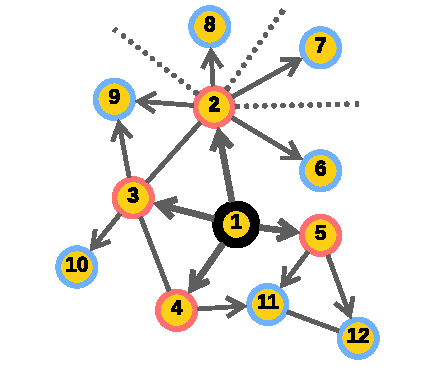
\includegraphics[width=0.31\linewidth]{out/about-pruning-01.pdf}
  }
  \subfigure[Disregard hubs with degree $> 8$]{
    \label{fig:about-pruning--02}
    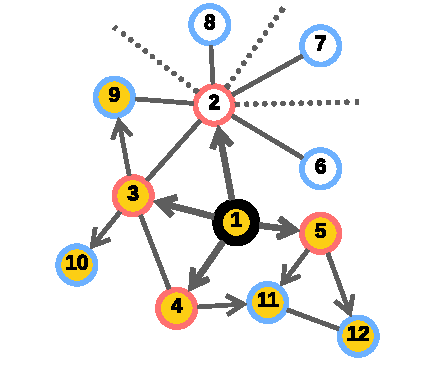
\includegraphics[width=0.31\linewidth]{out/about-pruning-02.pdf}
  }
  \subfigure[Disregard hubs with degree $> 4$]{
    \label{fig:about-pruning--03}
    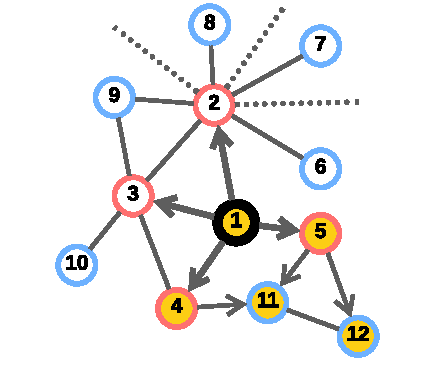
\includegraphics[width=0.31\linewidth]{out/about-pruning-03.pdf}
  } \\[-2ex]
  \caption{Illustration of our neighborhood-based link prediction approach, which disregards large hubs (first-order neighbors with high degree). The approach applies to each vertex in the graph. Here, we focus on the neighborhood of a vertex $1$ in the graph. The current vertex $1$ is outlined in black, its first-order neighbors in red, and its second-order neighbors in blue. Edge directions indicate traversal, with some second order vertices omitted for simplicity (dotted edges). (a) Depicts the standard approach, which considers all second-order neighbors of vertex $1$. (b) Presents our approach, which considers only second-order neighbors linked to $1$ through a small hub (degree $\leq 8$). This pruning reduces runtime and enhances prediction quality. (c) Illustrates our approach, where vertices with degree $> 4$ are considered large hubs.}
  \label{fig:about-pruning}
\end{figure*}

\begin{figure*}[hbtp]
  \centering
  \subfigure[Relative runtime (logarithmic scale), of each link prediction method]{
    \label{fig:adjust-mindegree--runtime}
    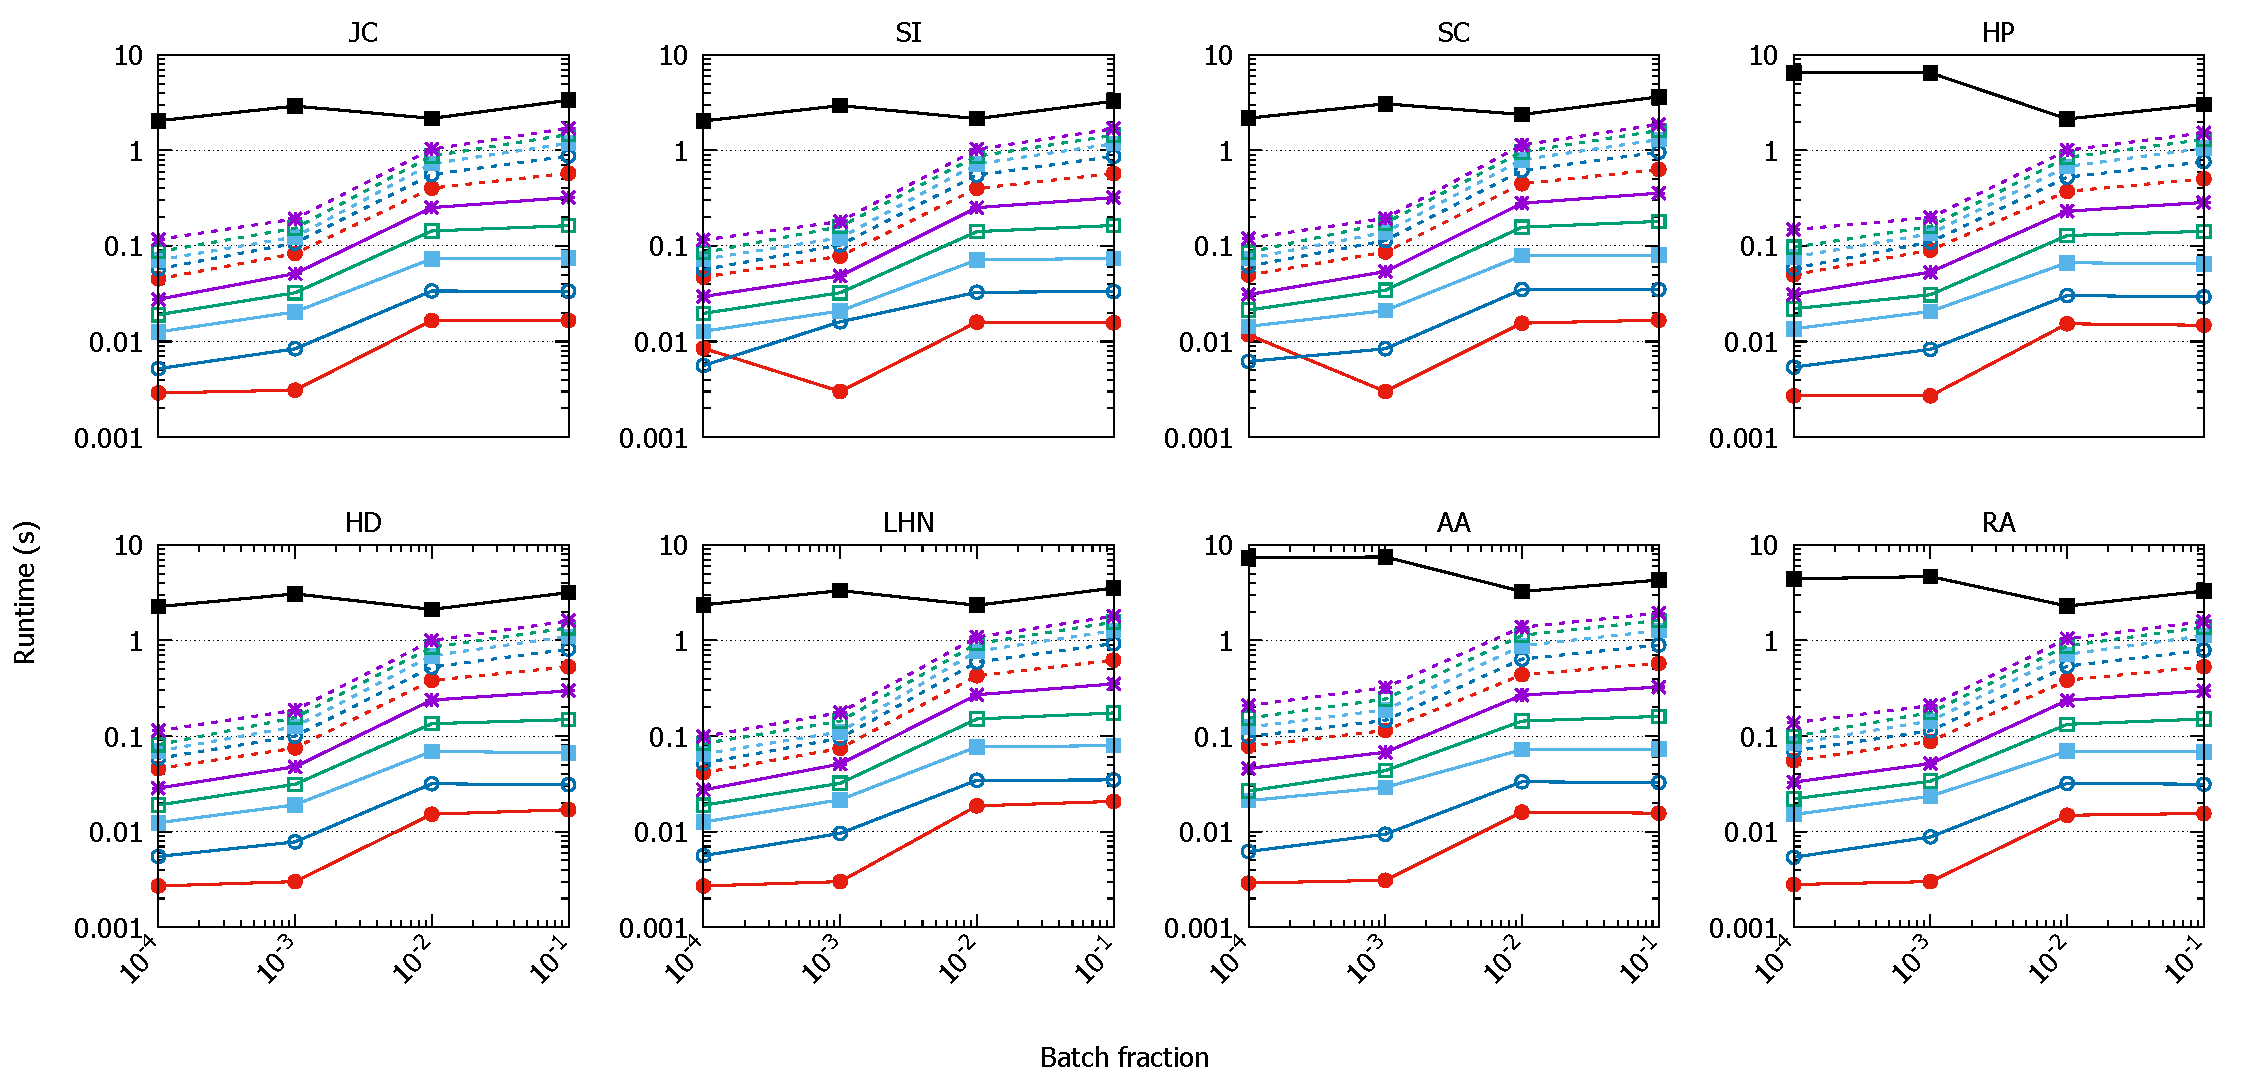
\includegraphics[width=0.98\linewidth]{out/adjust-mindegree-runtime.pdf}
  }
  \subfigure[F1 score of predicted links (logarithmic scale), of each link prediction method]{
    \label{fig:adjust-mindegree--precision}
    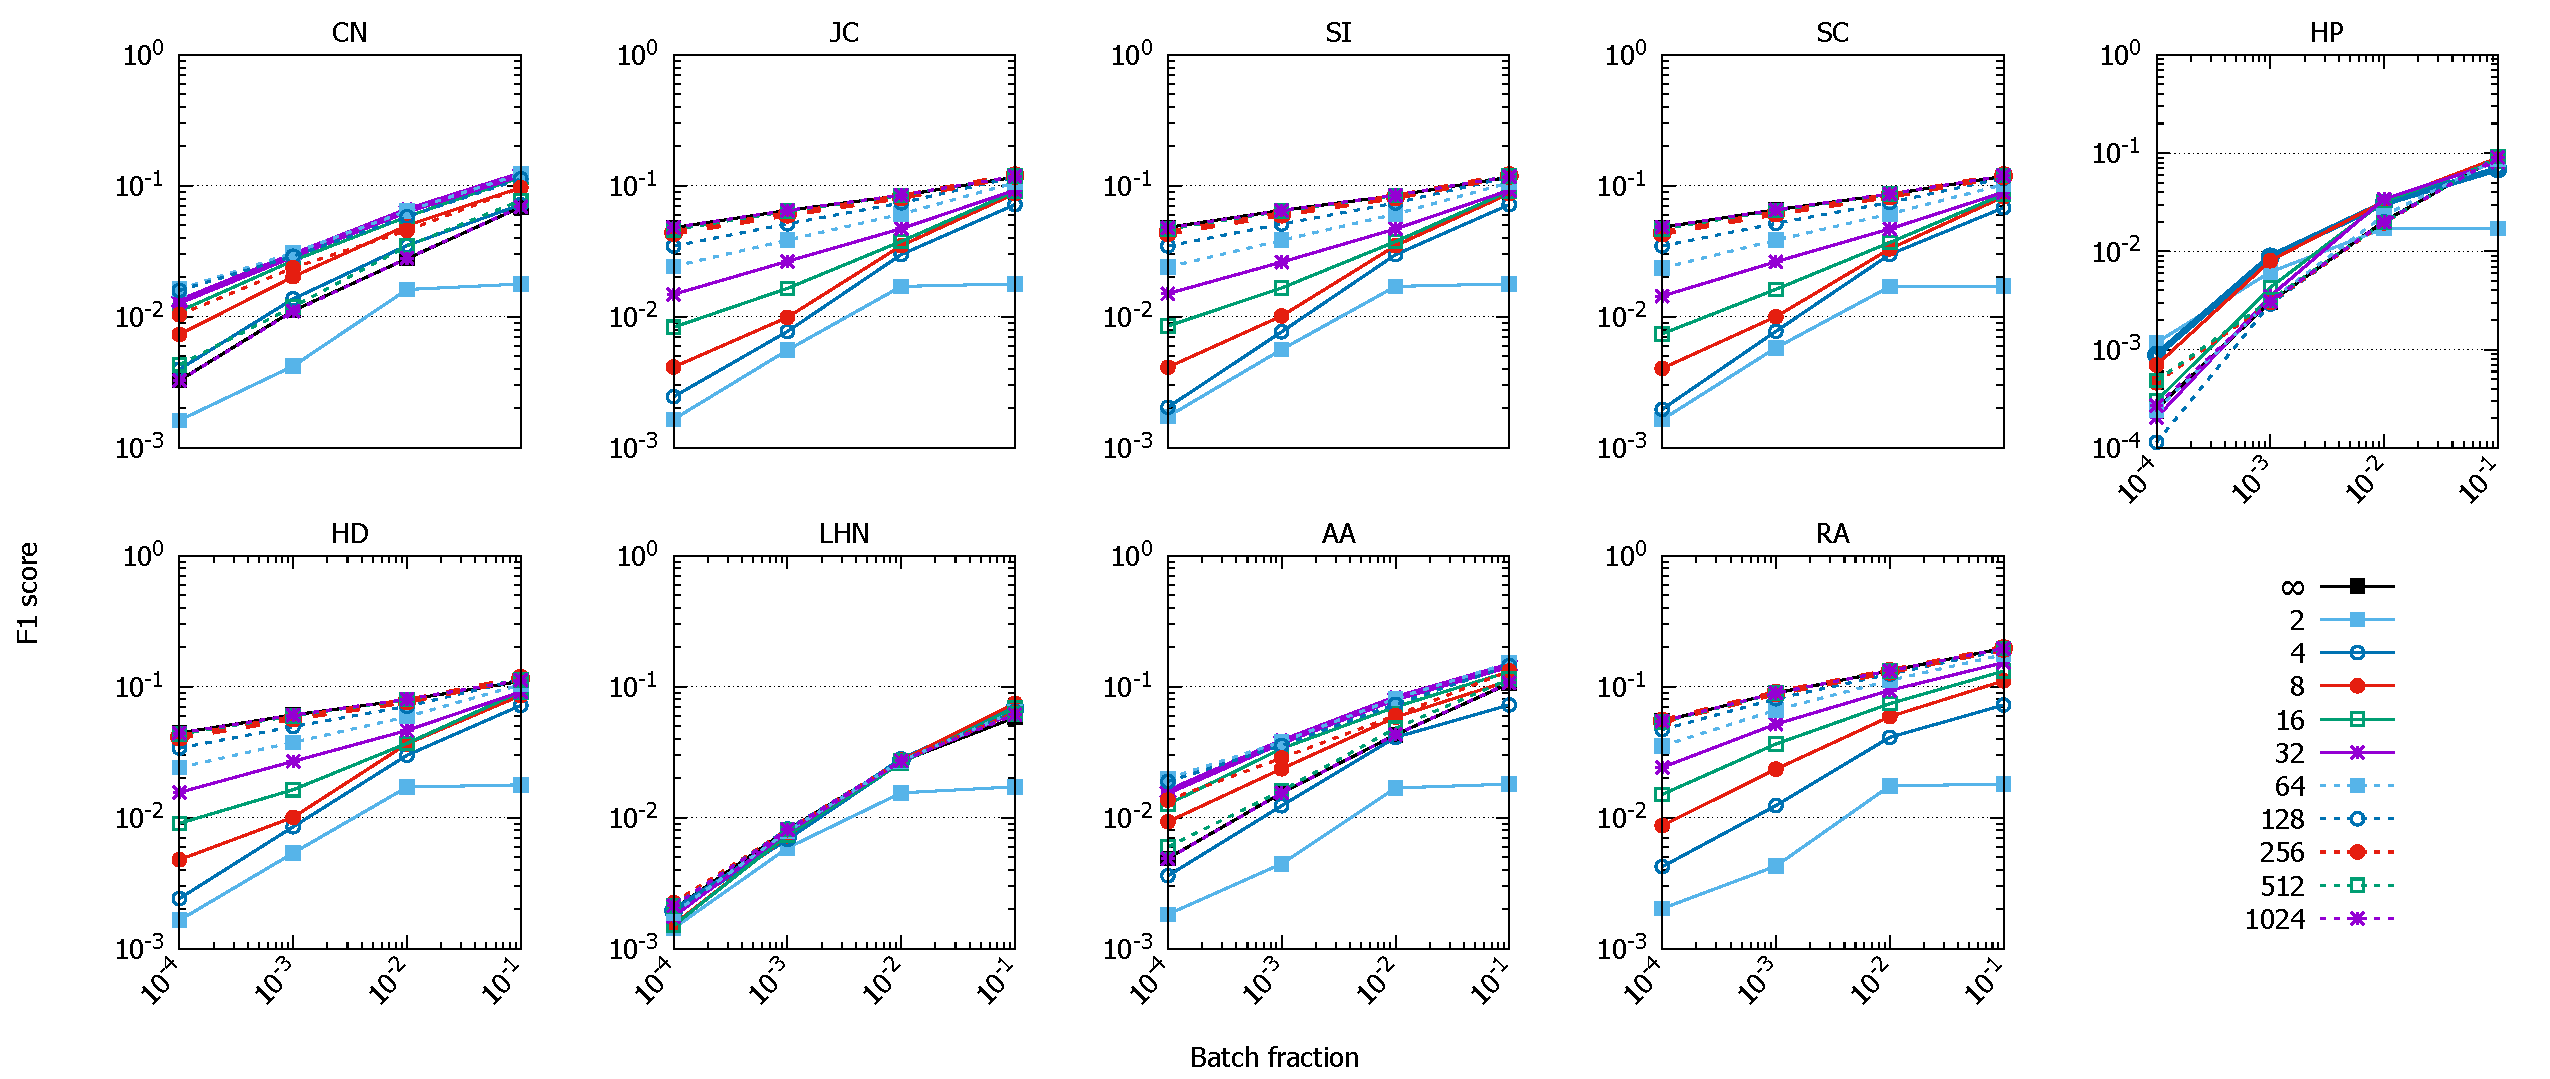
\includegraphics[width=0.98\linewidth]{out/adjust-mindegree-f1score.pdf}
  } \\[0ex]
  \caption{Impact of adjusting the \textit{MAX\_MEDIATOR\_DEGREE} from $2$ to $1024$ (in multiples of $2$), and to $\infty$, on the runtime (in seconds, log-scale), and precision of predicted links (in percentage, log scale), of each neighbor-based link prediction method, on batch sizes of $10^{-4}|E|$ to $0.1|E|$. The full form of each link prediction method is given in Section X.}
  \label{fig:adjust-mindegree}
\end{figure*}



\subsubsection{Local-moving phase of GVE-Leiden}

TODO.


\subsubsection{Refinement phase of GVE-Leiden}

TODO.


\subsubsection{Aggregation phase of GVE-Leiden}

TODO.




\subsection{Finding disconnected communities}

TODO.


\section{Evaluation}
\label{sec:evaluation}
\subsection{Experimental Setup}
\label{sec:setup}

\subsubsection{System used}

We use a server outfitted with two Intel Xeon Gold 6226R processors. Each processor comprises $16$ cores operating at $2.90$ GHz. Each core has a $1$ MB L1 cache, a $16$ MB L2 cache, and a shared L3 cache of $22$ MB. The system is set up with $376$ GB of system memory and has CentOS Stream 8 installed.\ok{}


\subsubsection{Configuration}

We employ 32-bit integers to represent vertex IDs and 32-bit floats for score computation. We utilize $32$ threads to match the system core count (unless specified otherwise). Compilation is carried out using GCC 8.5 and OpenMP 4.5.\ok{}


\subsubsection{Dataset}

The graphs used in our experiments are given in Table \ref{tab:dataset}. These are sourced from the SuiteSparse Matrix Collection \cite{suite19}. In the graphs, number of vertices vary from $3.07$ to $214$ million, and number of edges vary from $25.4$ million to $3.80$ billion. We ensure edges to be undirected and weighted with a default of $1$.


\subsubsection{Observed Graph generation}

To generate the observed graphs, we take each graph from the dataset and randomly remove $10^-4|E|$ to $0.1|E|$ edges from it --- where the endpoints of removed edges are chosen with uniformly probability.\ignore{For each batch size, we generate five random batch updates for averaging.}
The evaluation involves splitting ground-truth links ($E$) into observed ($E^O$) and unobserved ($E^U$) sets, using $E^O$ for known information and $E^U$ for algorithm evaluation \cite{arrar2023comprehensive}.
The majority of known studies apply ‘‘random division’’, namely $E^P$ is randomly drawn from $E$ \cite{zhou2021progresses}.
Although $|E^P|$ is generally unknown, an experiential and reasonable setting is  $|E^P| = 0.1 |E|$ because $10\%$ of links in the probe set are usually enough for us to get statistical solid results while the removal of $10\%$ of links will probably not destroy the structural features of the target network \cite{lu2015toward}.

\ignore{Are there no missing links in the original graphs?}

\begin{table}[hbtp]
  \centering
  \caption{List of $13$ graphs obtained SuiteSparse Matrix Collection \cite{suite19} (directed graphs are marked with $*$). Here, $|V|$ is the number of vertices, $|E|$ is the number of edges (after adding reverse edges), $D_{avg}$ is the average degree, and $|\Gamma|$ is the number of communities obtained with \textit{GVE-Leiden}.\ignore{In the table, B refers to a billion, M refers to a million and K refers a thousand.}}
  \label{tab:dataset}
  \begin{tabular}{|c||c|c|c|c|}
    \toprule
    \textbf{Graph} &
    \textbf{\textbf{$|V|$}} &
    \textbf{\textbf{$|E|$}} &
    \textbf{\textbf{$D_{avg}$}} &
    \textbf{\textbf{$|\Gamma|$}} \\
    % \textbf{$1 - \Gamma_G$} \\
    \midrule
    \multicolumn{5}{|c|}{\textbf{Web Graphs (LAW)}} \\ \hline
    indochina-2004$^*$ & 7.41M & 341M & 41.0 & 5.00K \\ \hline  % & \num{4.7e-4} & 2.9 GB
    uk-2002$^*$ & 18.5M & 567M & 16.1 & 43.1K \\ \hline  % & \num{9.6e-5} & 16 GB
    arabic-2005$^*$ & 22.7M & 1.21B & 28.2 & 3.80K \\ \hline  % & \num{5.5e-4} & 11 GB
    uk-2005$^*$ & 39.5M & 1.73B & 23.7 & 21.2K \\ \hline  % & \num{9.6e-5} & 16 GB
    webbase-2001$^*$ & 118M & 1.89B & 8.6 & 2.77M \\ \hline  % & \num{7.3e-7} & 18 GB
    it-2004$^*$ & 41.3M & 2.19B & 27.9 & 5.24K \\ \hline  % & \num{3.8e-4} & 19 GB
    sk-2005$^*$ & 50.6M & 3.80B & 38.5 & 3.75K \\ \hline  % & \num{5.8e-4} & 33 GB
    \multicolumn{5}{|c|}{\textbf{Social Networks (SNAP)}} \\ \hline
    com-LiveJournal & 4.00M & 69.4M & 17.4 & 2.33K \\ \hline  % & \num{7.9e-4} & 480 MB
    com-Orkut & 3.07M & 234M & 76.2 & 33 \\ \hline  % & \num{6.7e-2} & 1.7 GB
    \multicolumn{5}{|c|}{\textbf{Road Networks (DIMACS10)}} \\ \hline
    asia\_osm & 12.0M & 25.4M & 2.1 & 2.56K \\ \hline  % & \num{8.4e-4} & 200 MB
    europe\_osm & 50.9M & 108M & 2.1 & 3.61K \\ \hline  % & \num{6.6e-4} & 910 MB
    \multicolumn{5}{|c|}{\textbf{Protein k-mer Graphs (GenBank)}} \\ \hline
    kmer\_A2a & 171M & 361M & 2.1 & 19.4K \\ \hline  % & \num{9.4e-5} & 3.2 GB
    kmer\_V1r & 214M & 465M & 2.2 & 8.60K \\ \hline  % & \num{3.2e-4} & 4.2 GB
  \bottomrule
  \end{tabular}
\end{table}
% We convert directed graphs (marked with $*$) to undirected by duplicating edges in the reverse direction, and set the weight of each edge to $1$. and $F_{size}$ is size of the \textit{MatrixMarket} file





\subsection{Comparative Performance Evaluation}
%% Performance Comparison

In this section, we compare the performance of our approach, i.e., disregarding large hubs, and compare it with the default approach. We does this for observed graphs based on each graph in the dataset, with $10^-2|E|$ to $0.1|E|$ edges removed (the endpoints of removed edges are chosen with uniformly probability, as mentioned above), and predict the same number of edges with both approaches. For each observed graph, we predict links using the default approach, and our approach with suitable $MAX\_MEDIATOR\_DEGREE$, as identified in Section X. In Figures X, Y, and Z, we plot the runtimes, speedup, and precision respectively of only the best approach for each graph (both in terms of precision and runtime). In the figures, the labels indicate the acronyms of the similarity metric used, followed by the value of $MAX\_MEDIATOR\_DEGREE$ ($\Pi$) parameter setting (i.e., the label $HP4$ stands for the Hub Promoted similarity metric, with a $MAX\_MEDIATOR\_DEGREE$ of $4$, i.e., we avoid first order neighbors with degree greater than $4$). Note that a $MAX\_MEDIATOR\_DEGREE$ of $\infty$ is essentially the default/baseline approach. As Figures X, Y, and Z show, our approach is on average X times faster than the baseline/default approach, while predicting links with on average X\% higher precision. On the \textit{sk-2005} graph with $0.1|E|$ edges removed, our approach achieves a link prediction rate of X edges/s, and a processing rate of Y edges/s.

Although $|E^P|$ is generally unknown, an experiential and reasonable setting is  $|E^P| = 0.1 |E|$ because $10\%$ of links in the probe set are usually enough for us to get statistical solid results while the removal of $10\%$ of links will probably not destroy the structural features of the target network \cite{lu2015toward}.

\ignore{What does precision mean in the plots? \% of matching links with ground truth? How many ground truth links were missed?}

\ignore{Explain the confusion y-axis on precision.}

\ignore{Sizes of graphs are large so running other approaches (\Pi) is expensive.}

\ignore{What is the processing / prediction rate? (by predicted edges, and by number of edges in the graph)}

\ignore{Comparison with baseline approach ($\infty$), i.e., exploring all possible/reachable pairs at distance 2, and quickly computing intersection, scores, adding to heap, and merging across threads. Explain with figure in approach.}

\ignore{Why not showcase 0.01 E and 0.1 E, and remove the other plots?}

\ignore{Runtime + speedup + precision for $0.1|E|$.
Lu et al. \cite{lu2015toward} use precision.}

\ignore{Why is precision low?}
\ignore{Why precision on road networks and protein k-mer graphs low? (low average degrees)}
\ignore{It is possible that our algorithm only explores one type of connection, but the networks have various types of connections.}
\ignore{Quantifying a network's link predictability allows us to (i) evaluate predictive algorithms associated with the network, (ii) estimate the extent to which the organization of the network is explicable, and (iii) monitor sudden mechanistic changes during the network's evolution. The hypothesis of this paper is that a group of links is predictable if removing them has only a small effect on the network's structural features. We introduce a quantitative index for measuring link predictability and an algorithm that outperforms state-of-the-art link prediction methods in both accuracy and universality. This study provides fundamental insights into important scientific problems and will aid in the development of information filtering technologies \cite{lu2015toward}.}
\ignore{Are there no missing links in the original graphs?}
\ignore{Arent graphs heterogeneous? Why one method works?}
\ignore{Why do these methods perform well?}

\ignore{Can you show details plots? No.}

% Figure X shows the average runtime of link prediction with degree threshold $D$ of $4$, $8$, $16$, and $32$. Increasing $D$ increases runtime by a small amount, due to increase second-degree neighbor exploration. Increasing/decreasing the batch size however does not have an effect on runtime, as the algorithm must continue to explore possible links with higher scores even if batch/prediction size $B$ edges have been added to the prediction list. Note that runtime for link prediction with JC/HP similarity scores is nearly identical. On a batch size of $0.1 |E|$, we compare the predicted links with the links in the original graphs (without edge deletions). We observe that HP-based link prediction with $D = 16$ obtains the highest average accuracy of $2.4\%$, while HP-based link prediction with $D = 4$ obtains the highest average precision of $6.4\%$. Given the vast set of potential predictions (${}_N C_2 - |E|$), achieving high accuracy and precision remains a challenge.

\begin{figure*}[hbtp]
  \centering
  \subfigure[Runtime in seconds (logarithmic scale) for link prediction using the best similarity measure, with \textit{IHub} and \textit{LHub} approaches]{
    \label{fig:input-large--runtime}
    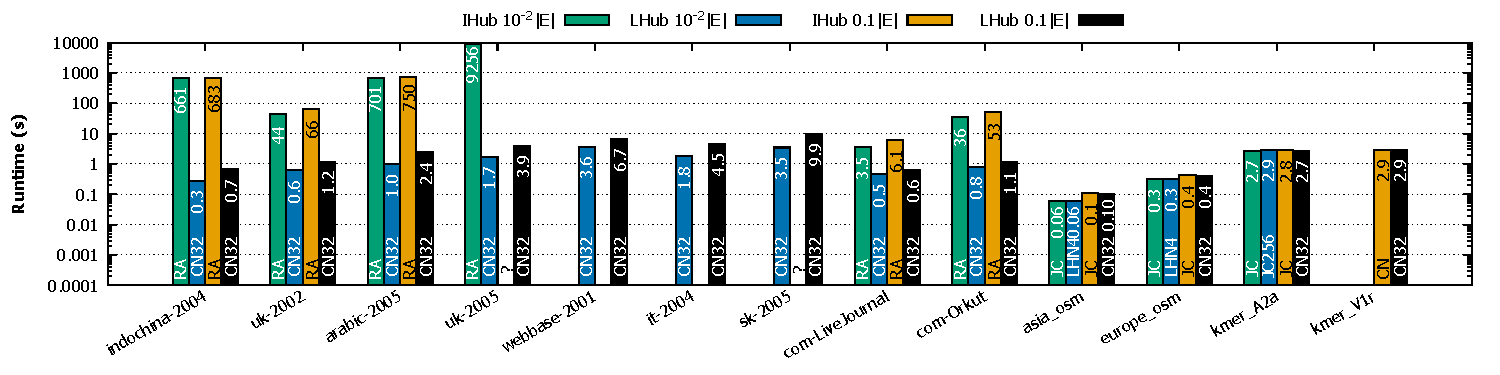
\includegraphics[width=0.98\linewidth]{out/input-large-runtime.pdf}
  }
  \subfigure[Speedup (logarithmic scale) for link prediction with the best similarity measure of \textit{LHub} approach, compared to \textit{IHub} approach]{
    \label{fig:input-large--speedup}
    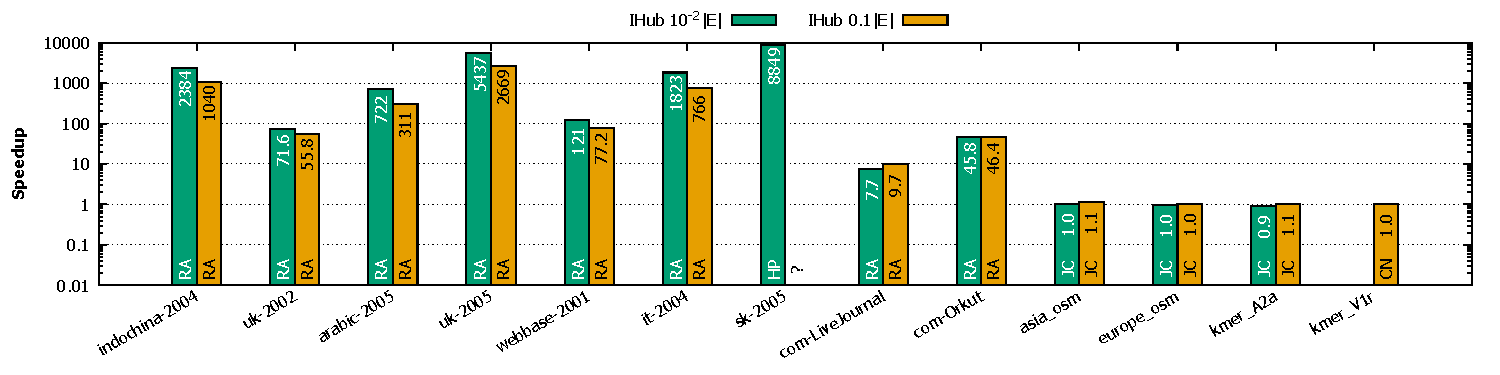
\includegraphics[width=0.98\linewidth]{out/input-large-speedup.pdf}
  }
  \subfigure[F1 score of predicted links (logarithmic scale), for link prediction using the best similarity measure, with \textit{IHub} and \textit{LHub} approaches]{
    \label{fig:input-large--f1score}
    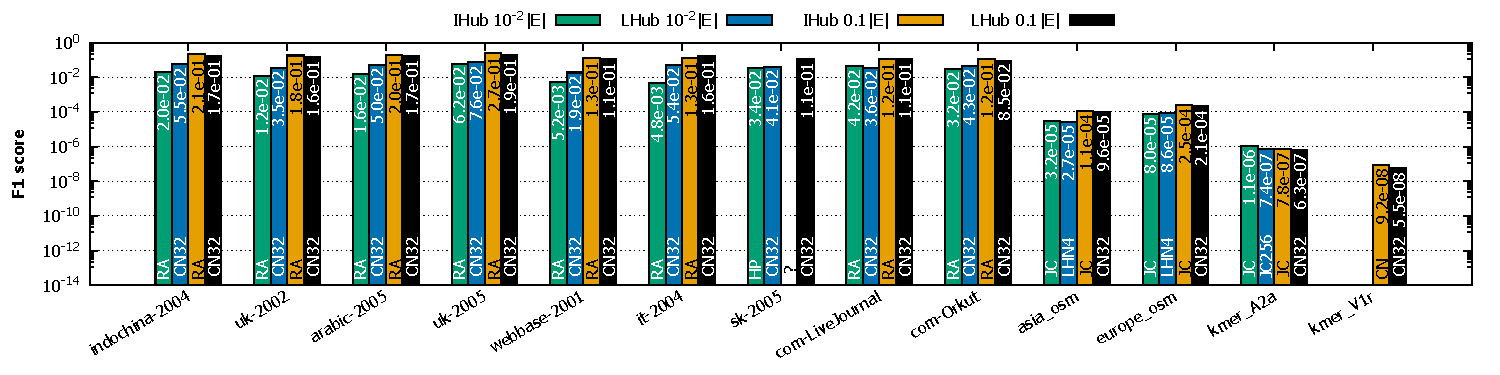
\includegraphics[width=0.98\linewidth]{out/input-large-f1score.pdf}
  } \\[-2ex]
  \caption{Runtime in seconds (log-scale), speedup (log-scale), and F1 score of predicted links (log-scale), for link prediction method using the best similarity measure, when attempting to predict $10^{-2}|E|$ to $0.1|E|$ unobserved edges $E^U$, for each graph in the dataset. For each similarity measure outlined in Section \ref{sec:metrics}, we attempt only the best hub limit $L_H$ parameter setting obtained in Section \ref{sec:select-limit} (for the \textit{LHub} approach), and then select the best among them, considering both the F1 score and runtime. Note that the numerical suffix added to the acronym of each link prediction method, with the \textit{LHub} approach, indicates the hub limit $L_H$ parameter setting.}
  \label{fig:input-large}
\end{figure*}

\begin{figure}[hbtp]
  \centering
  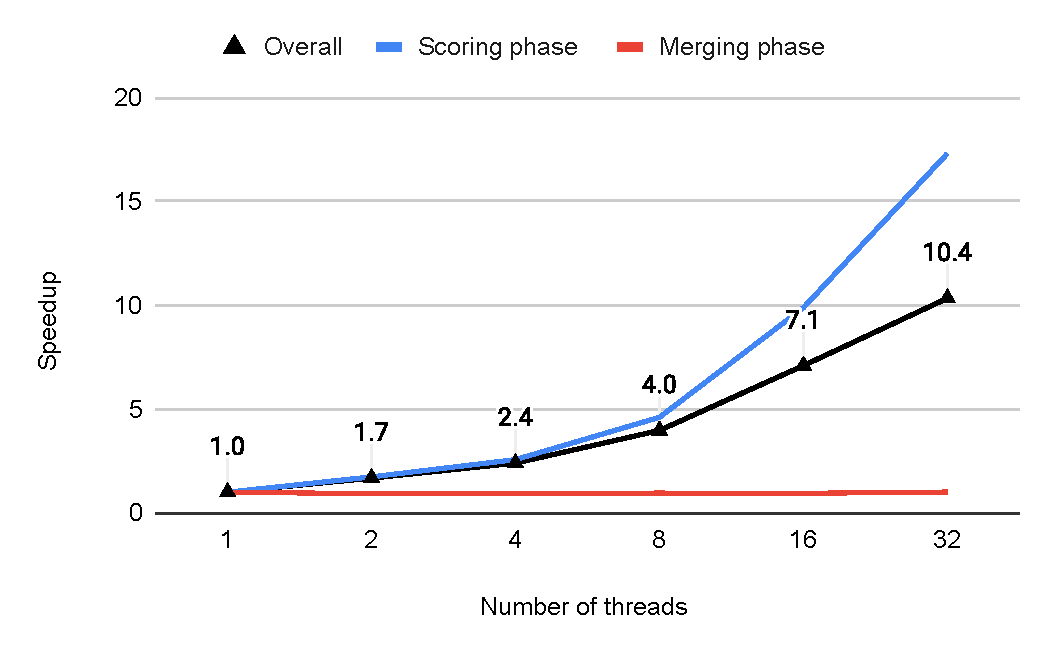
\includegraphics[width=0.98\linewidth]{out/strong-scaling-speedup.pdf} \\[-2ex]
  \caption{Overall speedup of our approach of \textit{Disregarding Large Hubs (DLH)} for link prediction, and its phases (obtaining edges with top-k scores per thread, and merging scores from each thread into a common scoreboard), with $10^{-2}|E|$ unobserved edges, with increasing number of threads (in multiples of 2). Increasing the number of threads causes work in the merging phase to increase,\ignore{thus} leading to a poor speedup.}
  \label{fig:strong-scaling}
\end{figure}





\subsection{Selecting Suitable Similarity Metric}

Extensive experiments \cite{ghasemian2020stacking} show that no known link predictor performs best or worst across all inputs \cite{zhou2021progresses}.\ignore{We expect a larger fraction of algorithms in the future studies will be designed for networks of particular types \cite{zhou2021progresses}.} In this section, we select a suitable similarity metric for link prediction for each type of graph. For this, we generate observed graphs from each graph in the dataset, such that $10^-4|E|$ to $0.1|E|$ edges are removed (the endpoints of removed edges are chosen with uniformly probability), and predict the same number of edges using the best approach for each observed graph (as identified in Section X).

In Figures X and Y, we plot the runtimes and precision of the best approach for each graph (both in terms of precision and runtime). As above, the labels in the figures indicate the acronyms of the similarity metric used, followed by the value of $MAX\_MEDIATOR\_DEGREE$ ($\Pi$) parameter setting. As Figures X, Y, and Z show, approach X is suitable for web graph. On a set of smaller graphs (not shown here), we observe that approach X is suitable for co-citation graphs.

\ignore{What does precision mean in the plots? \% of matching links with ground truth? How many ground truth links were missed?}

\ignore{Explain the confusion y-axis on precision.}

\ignore{Selecting best approach based on precision and runtime, for batch size $10^{-4}|E|$ to $0.1|E|$, and present the result. The runtime and precision of each method (appendix).}

\ignore{Sizes of graphs are large so running other approaches is expensive.}

\ignore{Why precision on road networks and protein k-mer graphs low? (low average degrees)}

\ignore{What we observe on our dataset? What we observe on smaller graphs?}

\ignore{Why the choice of best method appears to change with batch size?}





\subsection{Strong Scaling}

Finally, we assess the strong scaling performance of our optimized neighbor-based link prediction methods. In this analysis, we vary the number of thread from $1$ to $32$ in multiples of $2$ for each input graph, and measure the average time taken to predict $10^{-2}|E|$ links by Hub Promoted (HP), Leicht-Holme-Nerman (LHN), Adamic-Adar Coefficient (AA), and Resource Allocation (RA) based link prediction methods with the \textit{MAX\_MEDIATOR\_DEGREE} parameter set to $4$. The results are shown in Figure \ref{fig:strong-scaling}. It not only illustrates the overall scaling performance, but the also scaling of the two phases of each link prediction method, i.e., identifying edges with top-k scores in each thread (scoring phase), and combining the scores obtained by each thread to obtain the global top-k edges (merging phase). With $32$ threads, our optimized link prediction methods achieve an overall speedup of $7.2\times$ (with respect to sequential execution), indicating a performance increase of $1.5\times$ for every doubling of threads. The scalability is limited, as the cost of the merging phase increases with an increase in the number of threads. In fact, at $32$ threads, the merging phase obtains a speedup of $0.7\times$ (yes it is less than $1$\ignore{, as its runtime increases}), while the scoring phase achieves a speedup of $18.5\times$.

\ignore{Why is string scaling of our link prediction approach low? Why is it especially for the merging phase?}

\begin{figure*}[hbtp]
  \centering
  \subfigure[Runtime]{
    \label{fig:input-small--runtime}
    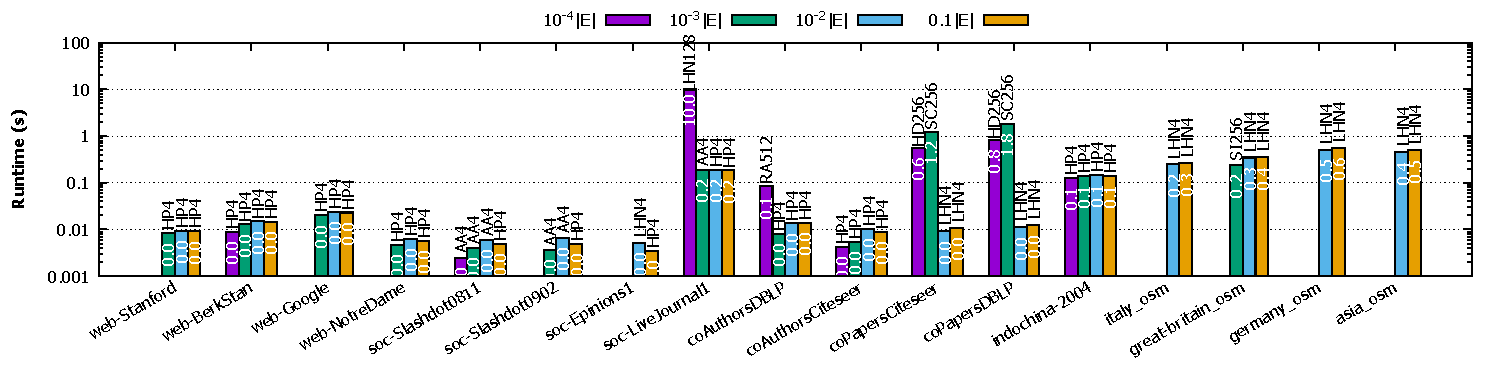
\includegraphics[width=0.98\linewidth]{out/input-small-runtime.pdf}
  }
  \subfigure[Precision]{
    \label{fig:input-small--precision}
    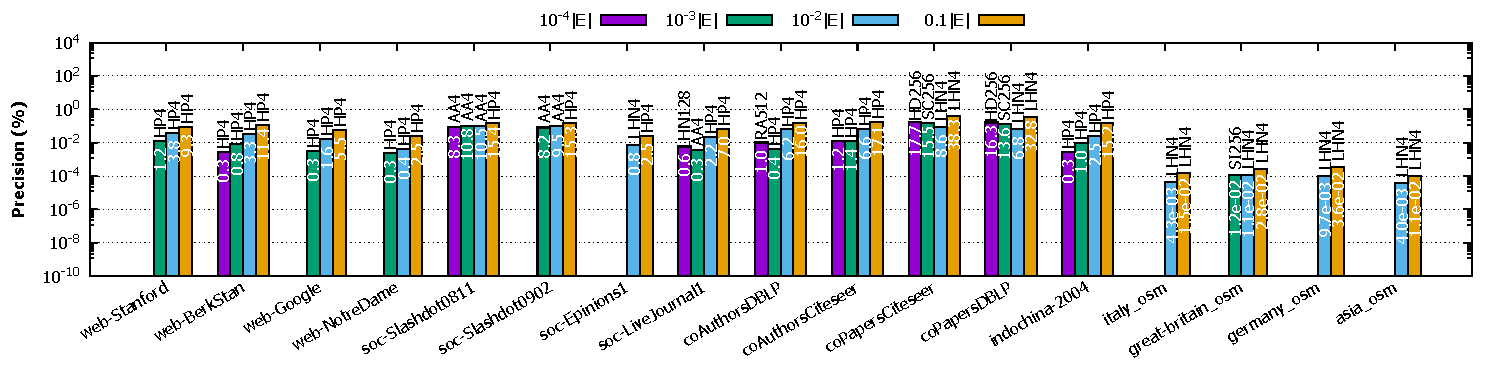
\includegraphics[width=0.98\linewidth]{out/input-small-precision.pdf}
  } \\[0ex]
  \caption{TODO. Input small.}
  \label{fig:input-small}
\end{figure*}



\section{Conclusion}
\label{sec:conclusion}
Link prediction aims to anticipate the existence of missing/future connection between nodes based on known interactions and network structure \cite{arrar2023comprehensive}. Similarity measures are commonly used for their simplicity, interpretability \cite{pai2019netdx, barbieri2014follow}, and computational efficiency \cite{garcia2014link}. Further, they are often combined with other approaches \cite{kumari2022supervised, abuoda2020link, pai2019netdx}, such as ensemble learning \cite{zhou2012ensemble}.

However, evaluating these algorithms on large networks is crucial for accurate insights \cite{zhou2021progresses, zhou2021experimental}. Many works in this field focus on small \cite{guo2019node, rafiee2020cndp, mumin2022efficient, papadimitriou2012fast, vega2021link, saifi2023fast, ferreira2019scalability, benhidour2022approach} to medium-scale graphs \cite{yang2015new, cui2016bounded, kalkanfinding, mohan2017scalable, wang2019link, bastami2019gravitation, shin2012multi, garcia2014link}, while parallelism becomes essential for larger networks. This technical report addresses both issues and introduces a heuristic for efficient computation. Further, a number of research studies \cite{gatadi2023lpcd, saifi2023fast, benhidour2022approach, mumin2022efficient, rafiee2020cndp, guo2019node, yang2015new, papadimitriou2012fast, wang2019link} and popular network analysis software (such as NetworKit \cite{staudt2016networkit} and igraph \cite{csardi2006igraph}), use the baseline approach, which computes similarity scores for all non-connected node pairs and predicts links based on the top-$k$ scores. Despite its simplicity, this approach incurs unnecessary computational costs as many node pairs lack common neighbors, and has a high time complexity\ignore{of $O(N^2D)$}.

In this report, we introduced the IHub approach, an enhanced parallel method that efficiently finds common neighbors and handles large graphs by tracking top-$k$ edges per-thread and later merging them globally.\ignore{This allows it to run on large graphs.} Additionally, we presented the LHub heuristic approach, which disregards large hubs. It is based on the notion that low-degree nodes contribute significant similarity among neighbors, in contrast to high-degree nodes (interestingly, this is similar to the idea behind the AA and RA similarity metrics). We then experimentally determined suitable hub limits for link prediction with each similarity metric.

Our results indicate that the LHub approach is, on average, over $963\times$ and $163\times$ faster than the IHub approach with $10^{-2}|E|$ and $0.1|E|$ unobserved edges, respectively. It achieves this speedup while predicting links with an average F1 score that is $61\%$ higher and $16\%$ lower, respectively --- meaning similar F1 scores without being too low or high. Notably, on the \textit{sk-2005} graph with $0.1|E|$ edges removed, LHub achieves a link prediction rate of $38.1M$ edges/s.

Moreover, RA metric shows superior performance in terms of F1 score and runtime on web graphs and social networks using the IHub approach. On road networks and protein k-mer graphs, JC similarity metric outperforms others with the IHub approach. With the LHub approach and $10^{-2}|E|$ unobserved edges, CN metric (hub limit $L_H$ of $32$) excels on web graphs and social networks, LHN metric (hub limit $L_H$ of $4$) performs best on road networks, and JC metric (hub limit $L_H$ of $256$) is optimal for protein k-mer graphs. However, with $0.1|E|$ unobserved edges, CN metric (hub limit $L_H$ of $32$) is the best across all graphs. LHub outperforms IHub, achieving higher F1 scores, particularly on web graphs and social networks.

When predicting $0.1|E|$ edges with the LHub approach, we observed that $63\%$ of the runtime is spent on the scoring phase, and especially higher on social networks, with high average degree. However, a significant portion is also dedicated to the merging phase, suggesting potential optimization opportunities for future work. In the strong scaling analysis, the LHub approach achieves a speedup of $12.4\times$ with 32 threads, indicating a performance increase of $1.7\times$ for every doubling of threads. However, scalability is constrained, particularly due to the merging phase. with a speedup of $0.7\times$ at 32 threads.

In the future, we want to explore optimizing quasi-local and global methods of similarity. While we explore second order neighbors in this report, our techniques can be extended to apply to higher order neighbors.

\ignore{Link prediction is essentially a compression problem, i.e. understanding the given network, and then predicting the missing links. As long as the network is not fully deterministic, one should not expect link prediction algorithms to be $100\%$ precise. Real-world networks lie somewhere between being completely deterministic, and completely random. It is possible that applying link prediction to multiple graphs of similar nature can help improve the accuracy of a link prediction algorithm. Note that explainabilty of link prediction algorithms is important.}


%% The acknowledgments section.
\begin{acks}
I would like to thank Prof. Kishore Kothapalli, Prof. K. Swarupa Rani, Ashwitha Gatadi, and Balavarun Pedapudi for their support.
\end{acks}

%% Bibliography style to be used, and the bibliography file.
\bibliographystyle{ACM-Reference-Format}
\bibliography{main}

\clearpage
\appendix
% \section{Additional Figures}
\begin{figure*}[hbtp]
  \centering
  \subfigure[Speedup of \textit{LHub} approach with different hub limits $L_H$]{
    \label{fig:adjust-overall--runtime}
    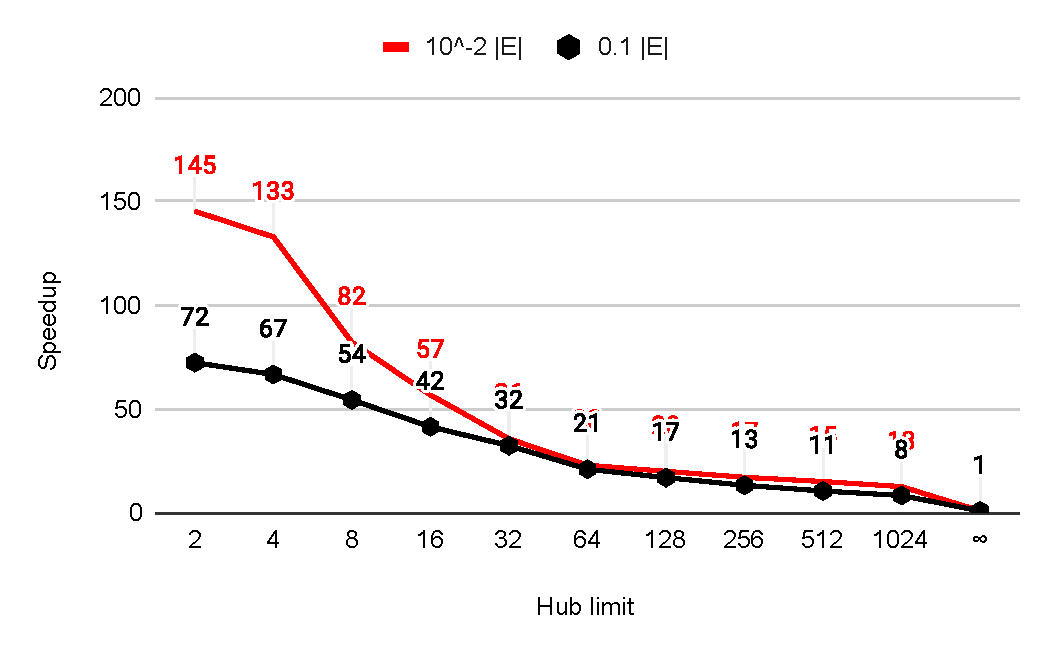
\includegraphics[width=0.48\linewidth]{out/adjust-overall-speedup.pdf}
  }
  \subfigure[F1 score of predicted links (logarithmic scale), with different hub limits $L_H$]{
    \label{fig:adjust-overall--precision}
    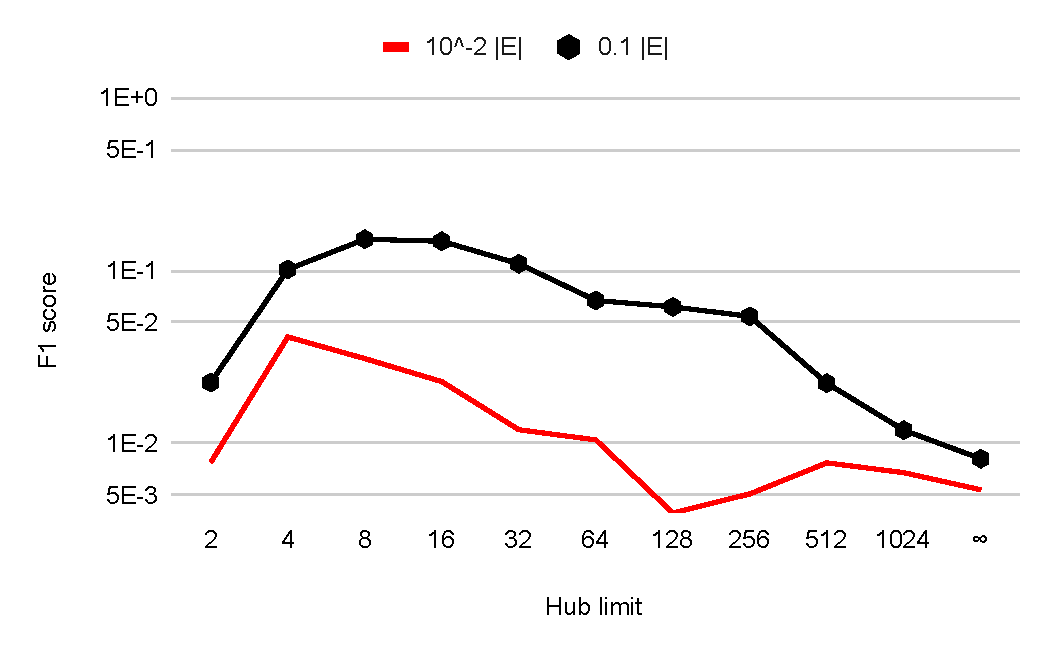
\includegraphics[width=0.48\linewidth]{out/adjust-overall-f1score.pdf}
  } \\[0ex]
  \caption{Overall impact of adjusting the hub limit $L_H$ from $2$ to $1024$ (in multiples of $2$), and to $\infty$, on the speedup and F1 score of predicted links (log scale), of neighbor-based link prediction methods, with the number of unobserved edges $E^U$ of $10^{-2}|E|$ and $0.1|E|$. Speedup is measured with respect to hub limit $L_H$ of $\infty$.\ignore{, using geometric mean of runtimes for link prediction using the LHub approach using all similarity scores given in Section \ref{sec:metrics}; while overall F1 score is obtained by taking the average.}}
  \label{fig:adjust-overall}
\end{figure*}

\begin{figure*}[hbtp]
  \centering
  \subfigure[Runtime in seconds (logarithmic scale) for link prediction using various similarity measures, with IHub approach]{
    \label{fig:standard2--runtime}
    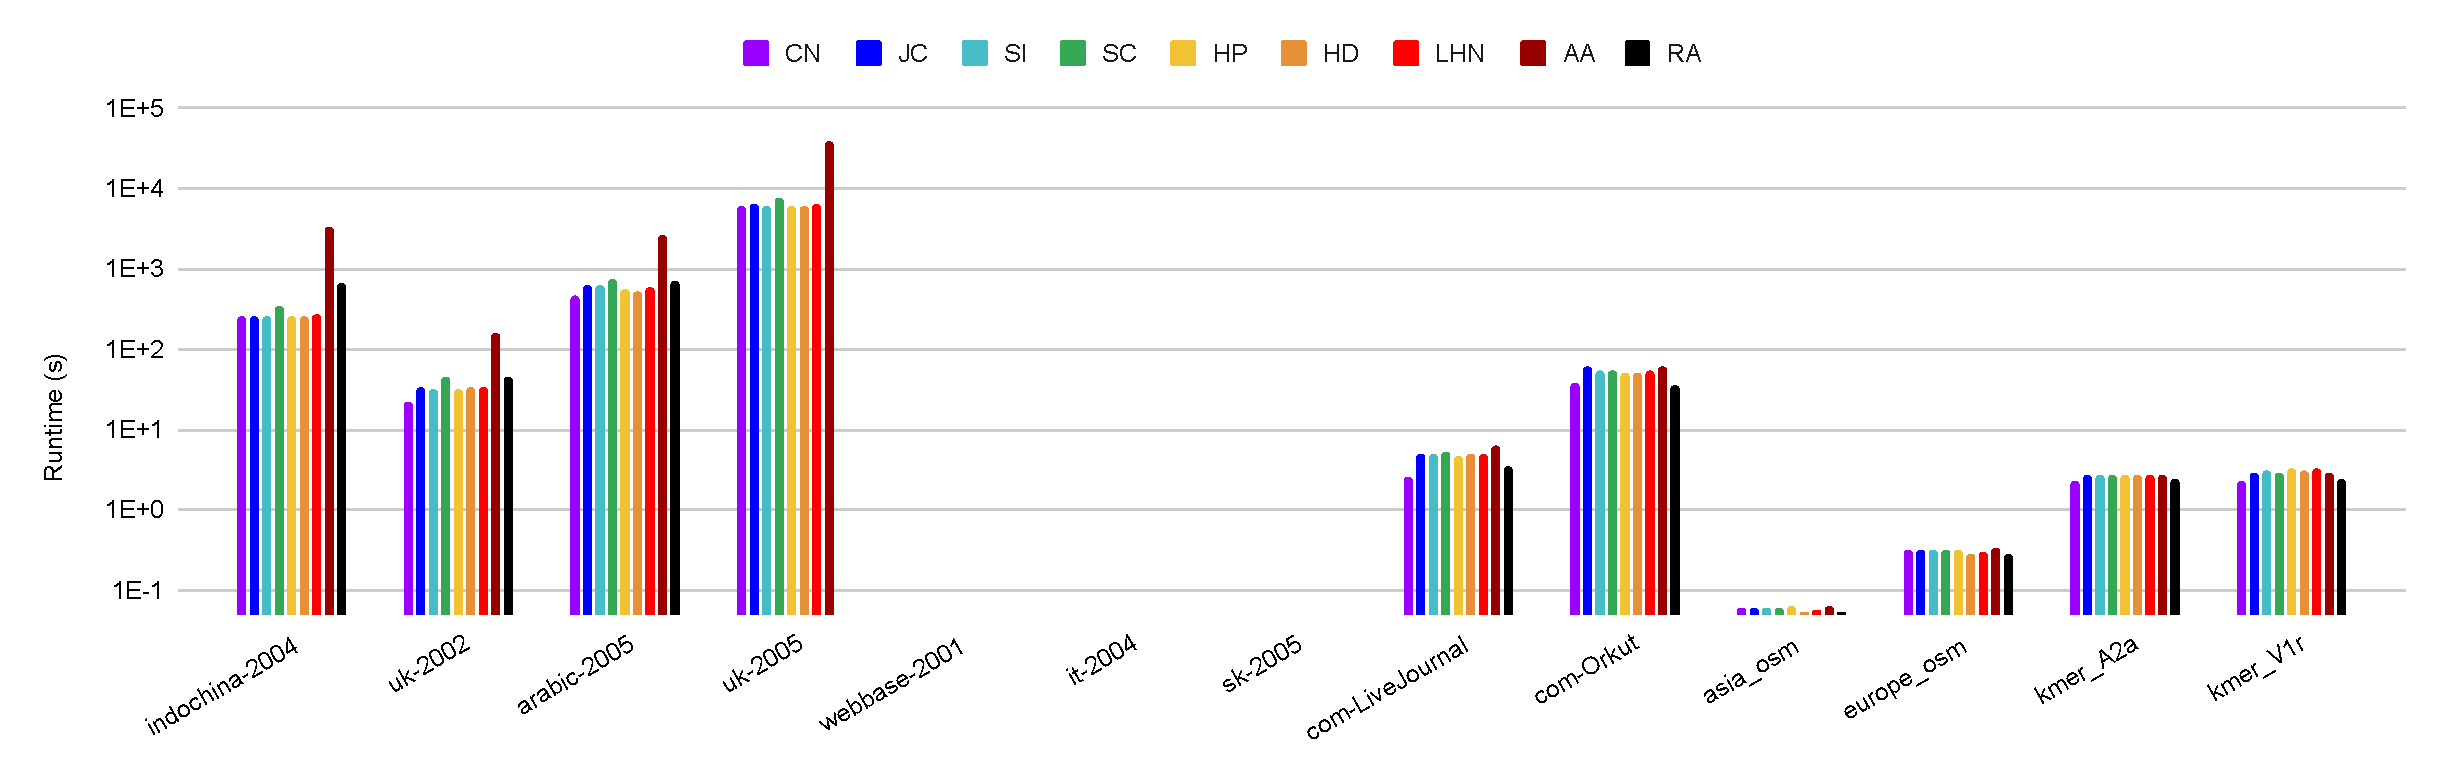
\includegraphics[width=0.98\linewidth]{out/standard2-runtime.pdf}
  }
  \subfigure[Precision of predicted links, in percentage (logarithmic scale), of the best neighborhood-based link prediction method]{
    \label{fig:standard2--f1score}
    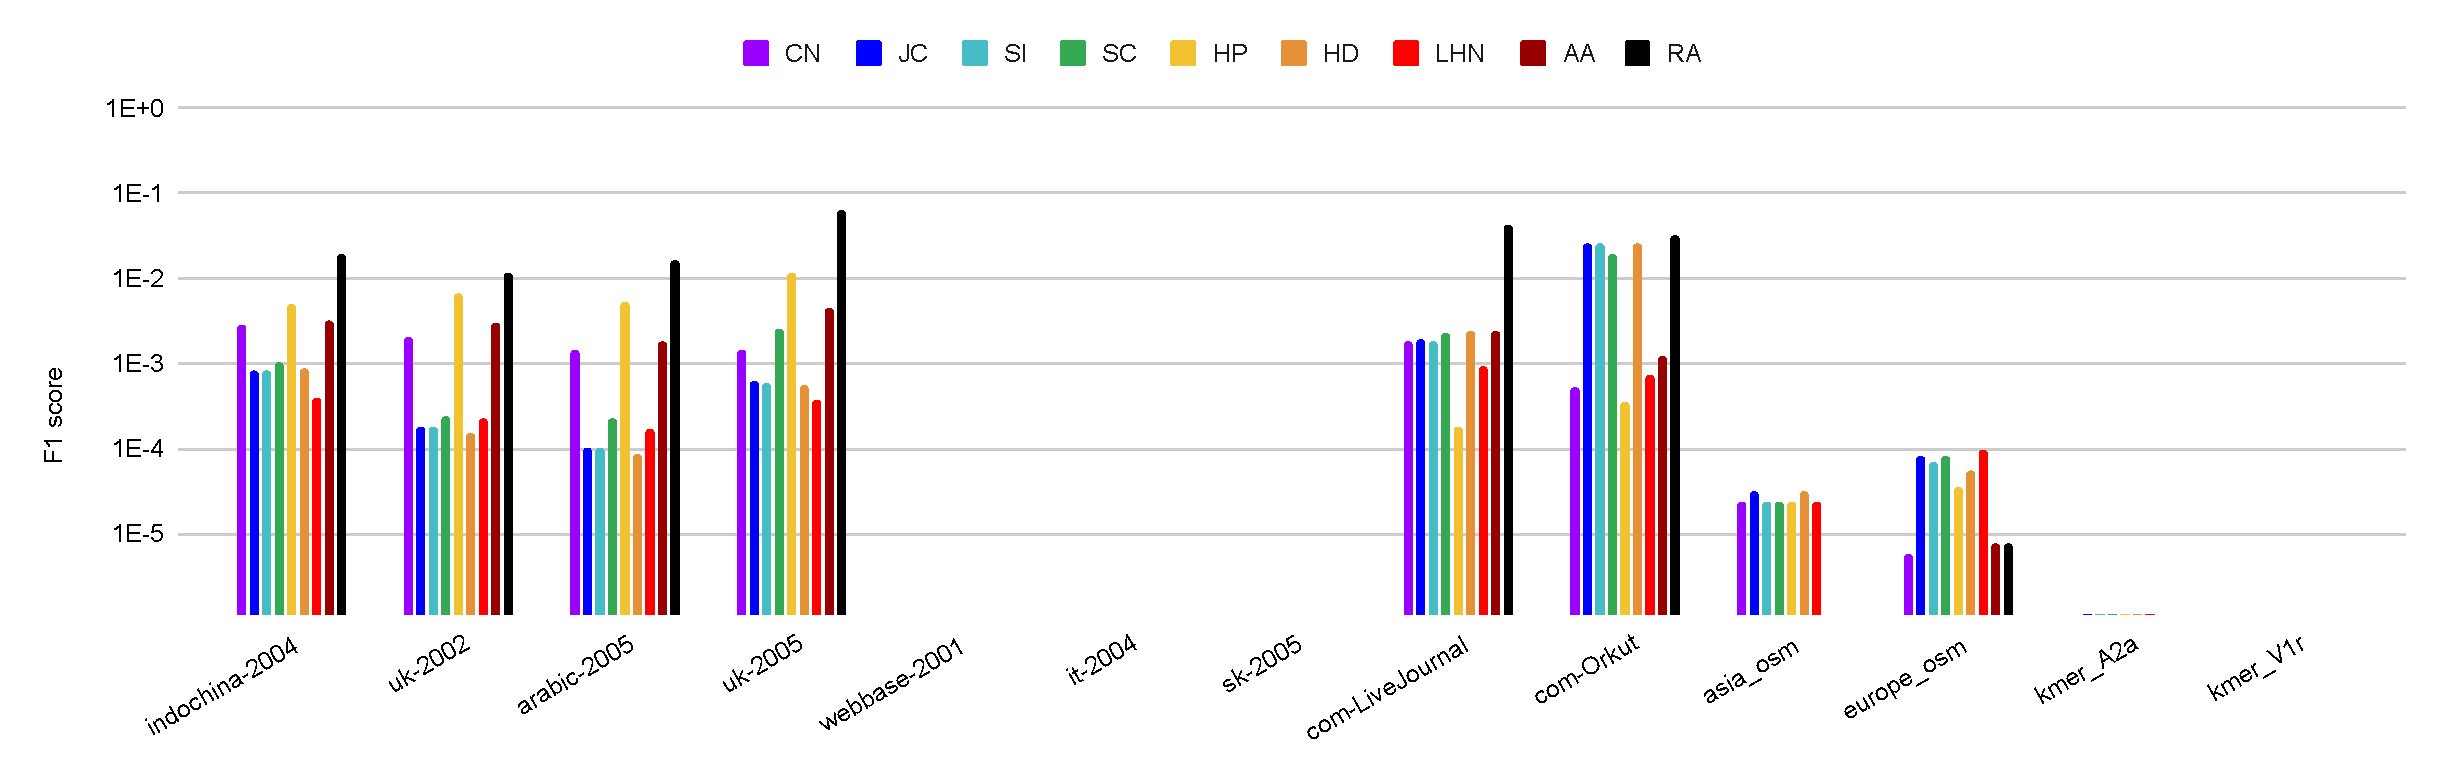
\includegraphics[width=0.98\linewidth]{out/standard2-f1score.pdf}
  } \\[-2ex]
  \caption{TODO. Runtime in seconds (log-scale), and precision of predicted links, in percentage (log-scale), of the best neighborhood-based link prediction method (considering both the precision and runtime), on batch sizes of $10^{-4}|E|$ to $0.1|E|$ for each graph in the dataset. None of the methods succeed in predicting ground-truth links for \textit{kmer\_V1r}, and for \textit{asia\_osm} and \textit{kmer\_A2a} on batch sizes of $10^{-4}|E|$ to $10^{-3}|E|$, and thus their results are not shown. Note that the numerical suffix added to the acronym of each link prediction method indicates the hub limit $L_H$ parameter setting.}
  \label{fig:standard2}
\end{figure*}

\begin{figure*}[hbtp]
  \centering
  \subfigure[Runtime in seconds (logarithmic scale) for link prediction using various similarity measures, with \textit{IBase} approach]{
    \label{fig:standard1--runtime}
    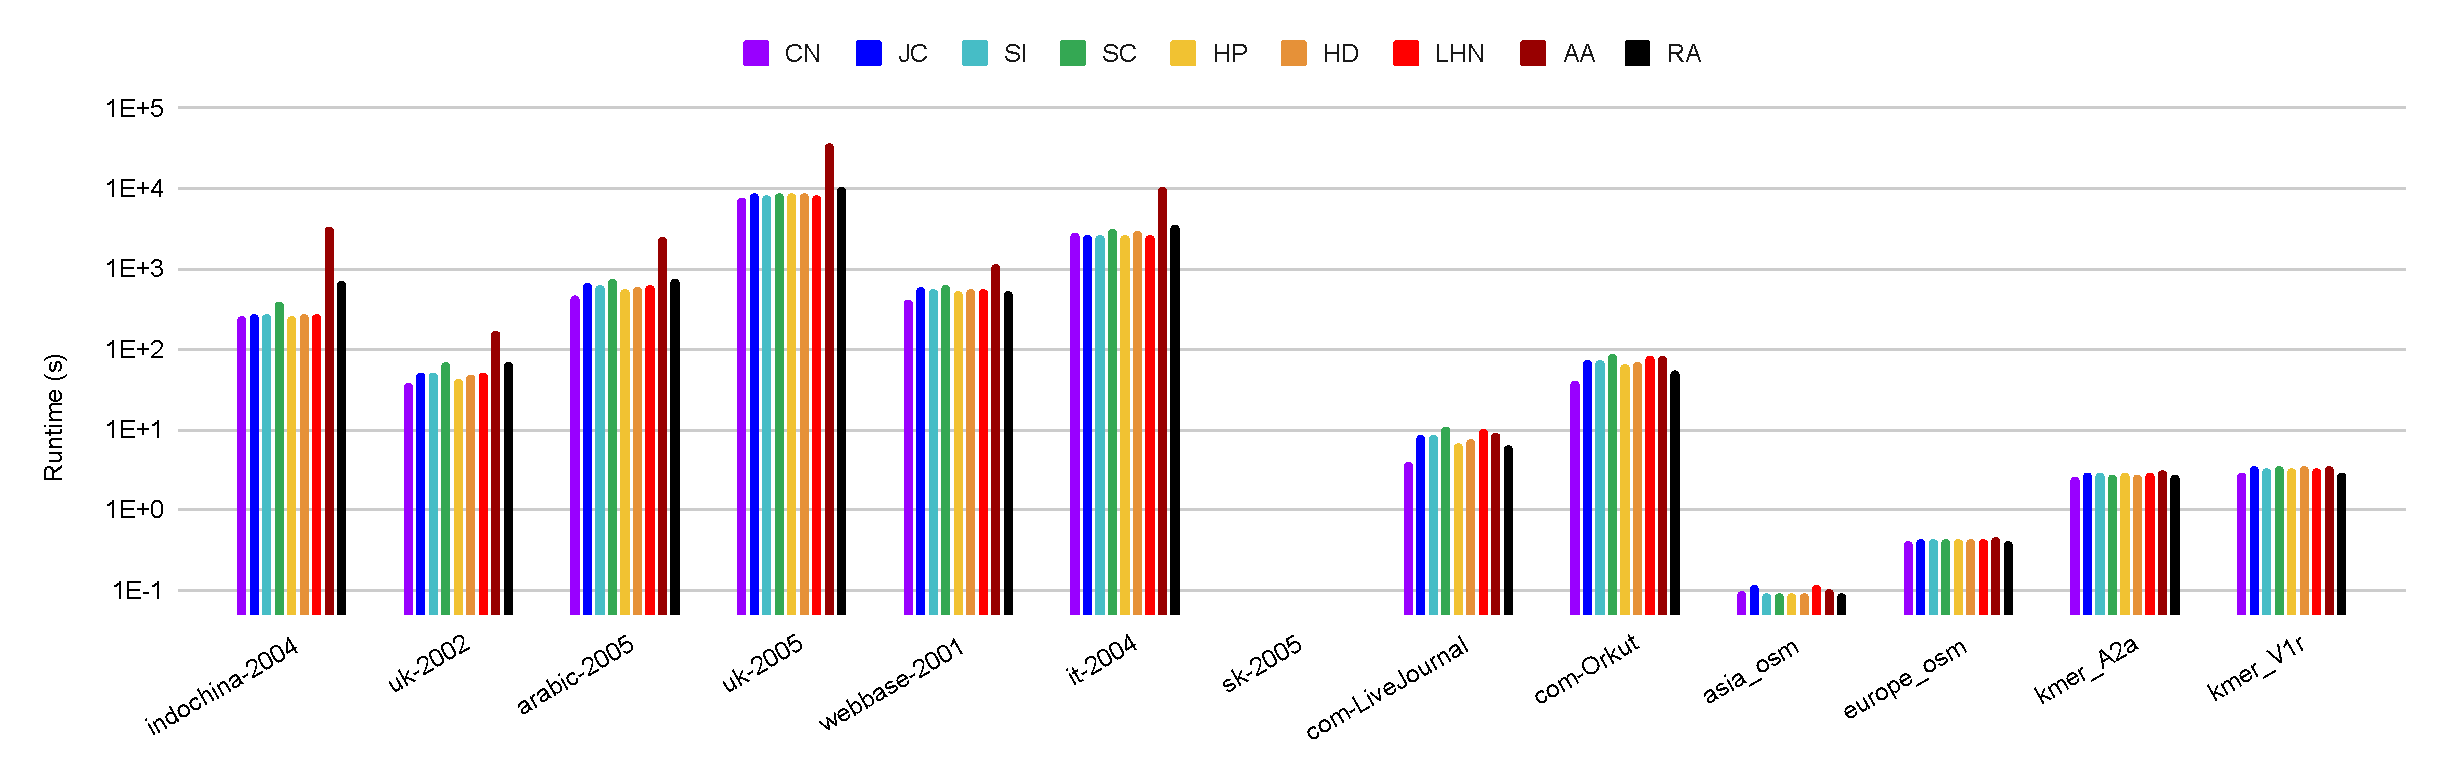
\includegraphics[width=0.98\linewidth]{out/standard1-runtime.pdf}
  }
  \subfigure[F1 score of predicted links (logarithmic scale) for link prediction using various similarity measures, with \textit{IBase} approach]{
    \label{fig:standard1--f1score}
    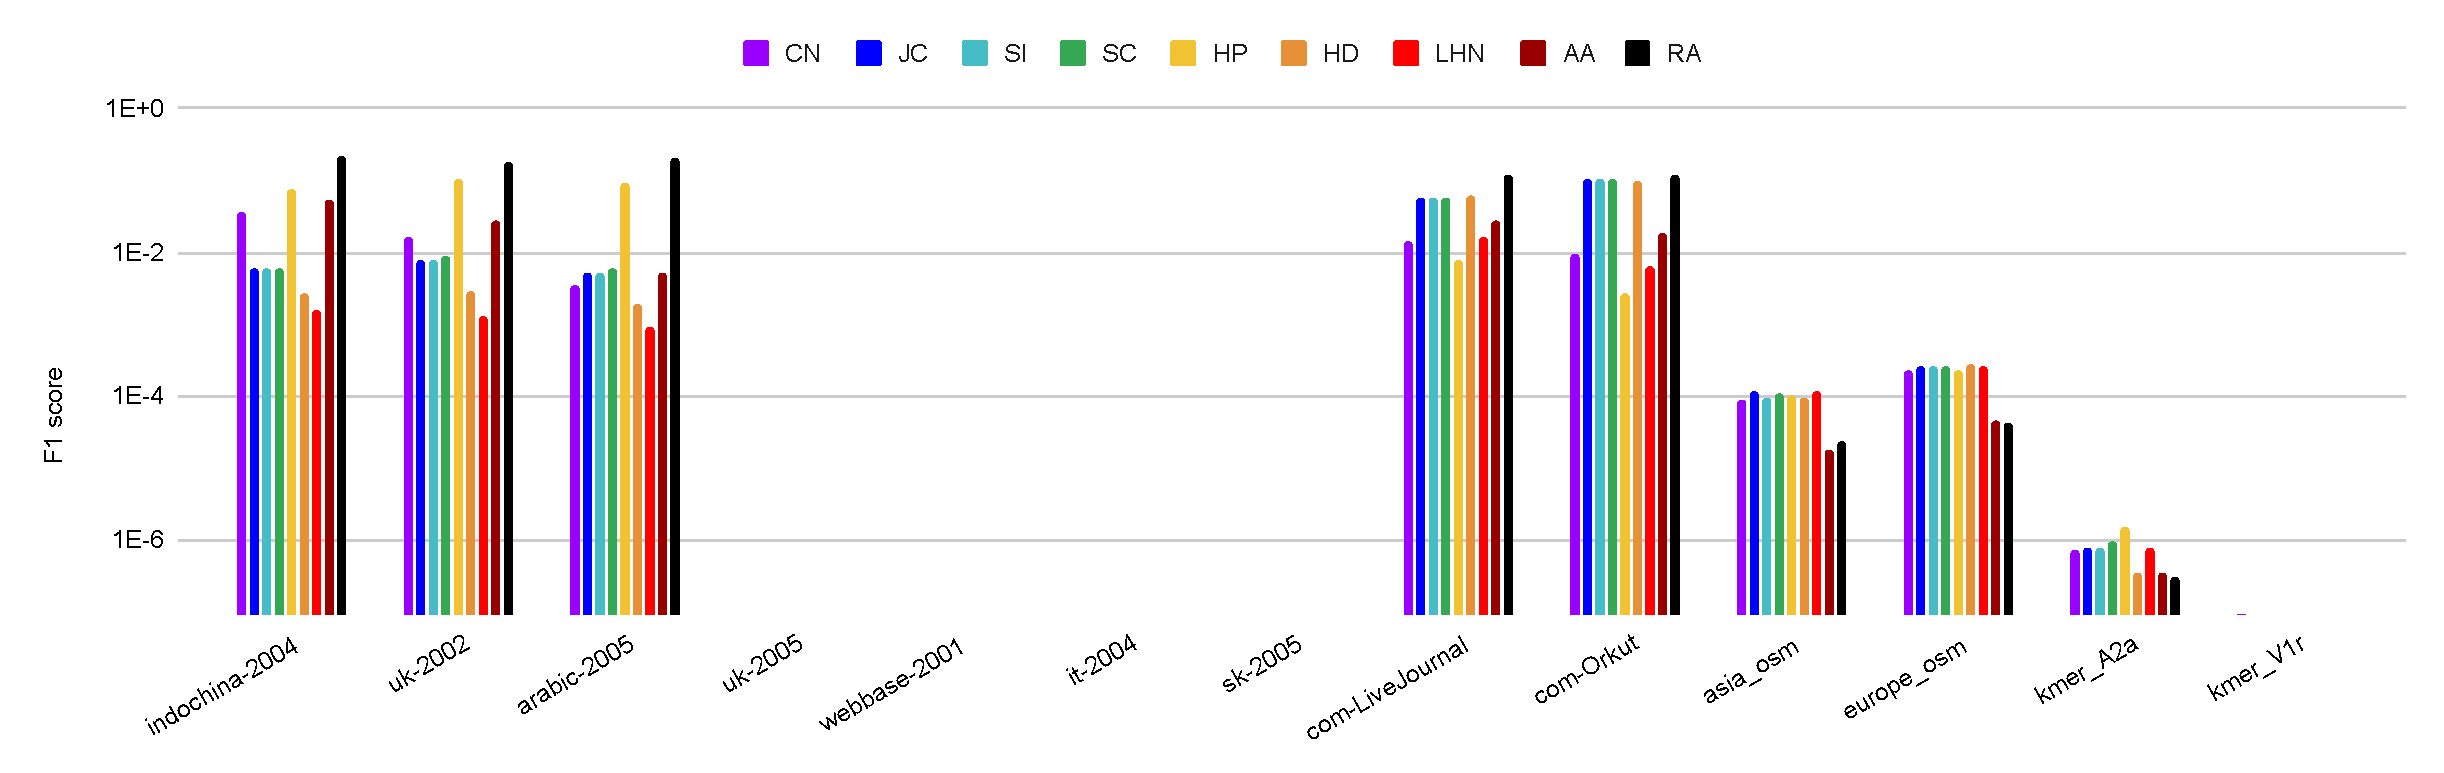
\includegraphics[width=0.98\linewidth]{out/standard1-f1score.pdf}
  } \\[-2ex]
  \caption{Runtime (log-scale) and F1 score (log-scale) for link prediction using various similarity measures with \textit{Improved Baseline (IBase)} approach, when attempting to predict $0.1|E|$ unobserved edges $E^U$ for each graph\ignore{in the dataset}.}
  \label{fig:standard1}
\end{figure*}

\begin{figure*}[hbtp]
  \centering
  \subfigure[Runtime in seconds (logarithmic scale) for link prediction using various similarity measures, with IHub approach]{
    \label{fig:pruned2--runtime}
    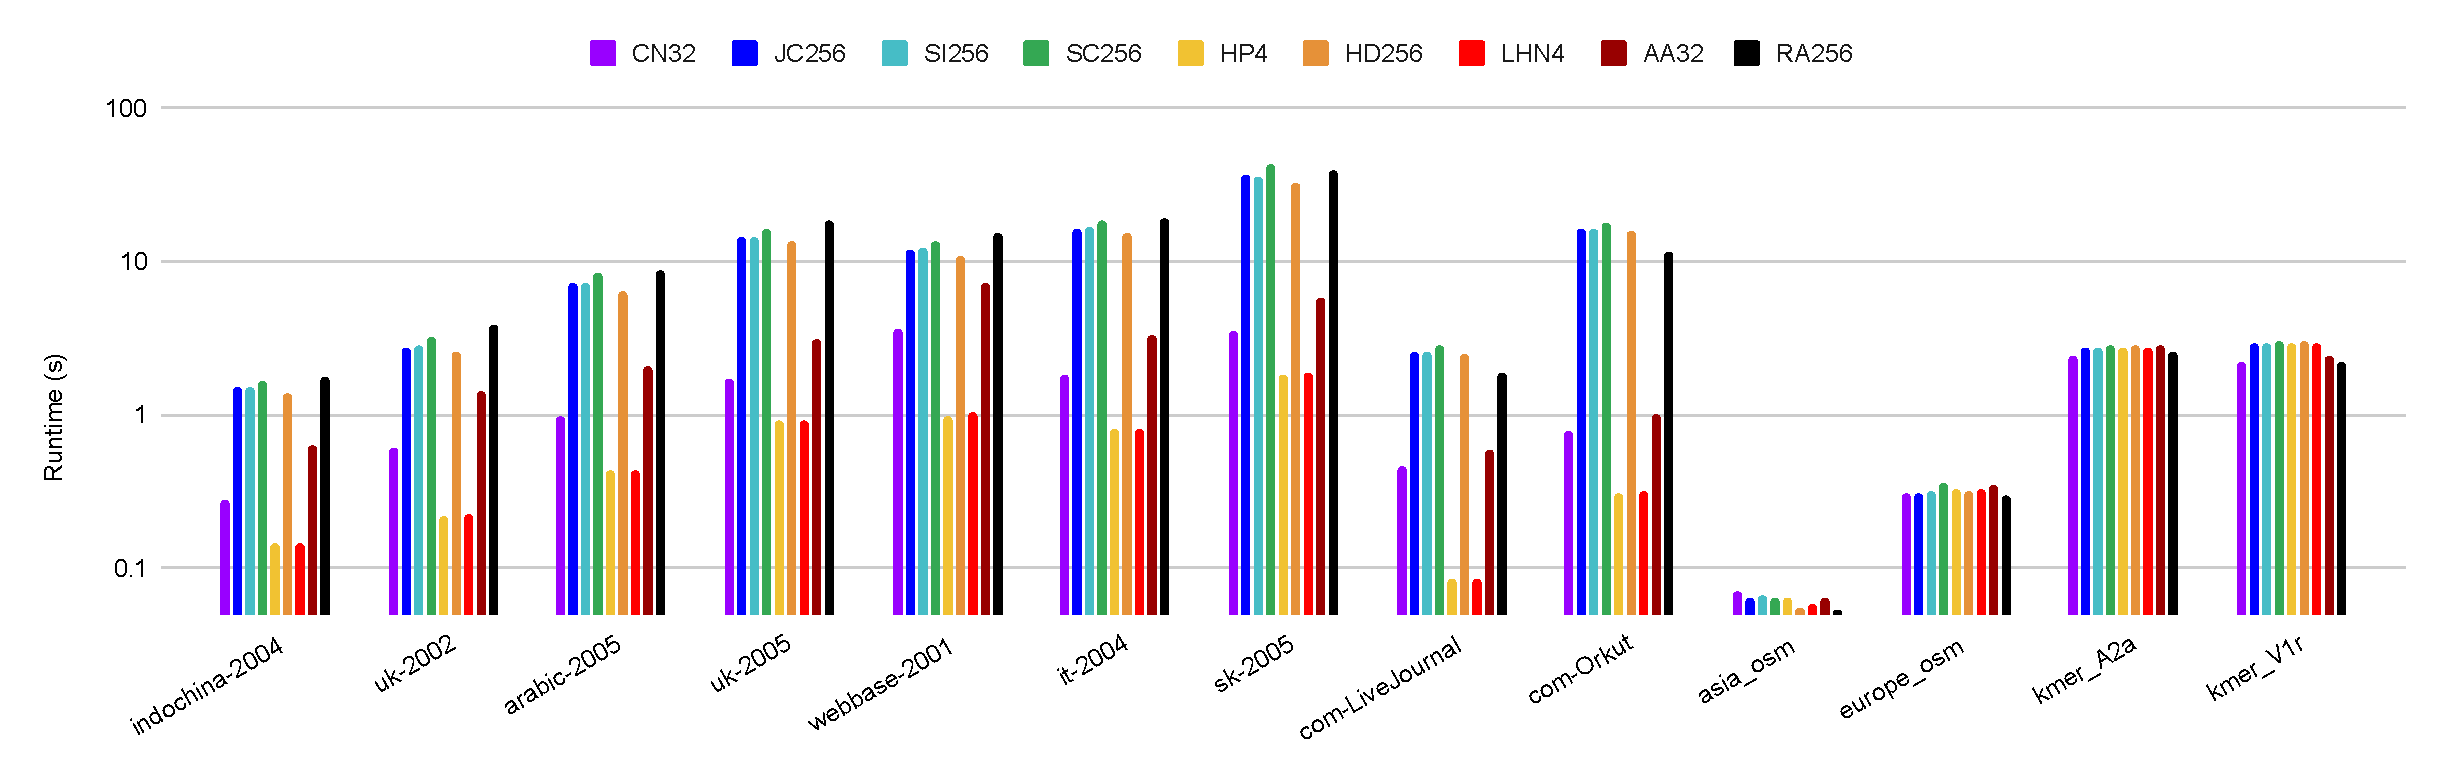
\includegraphics[width=0.98\linewidth]{out/pruned2-runtime.pdf}
  }
  \subfigure[Precision of predicted links, in percentage (logarithmic scale), of the best neighborhood-based link prediction method]{
    \label{fig:pruned2--f1score}
    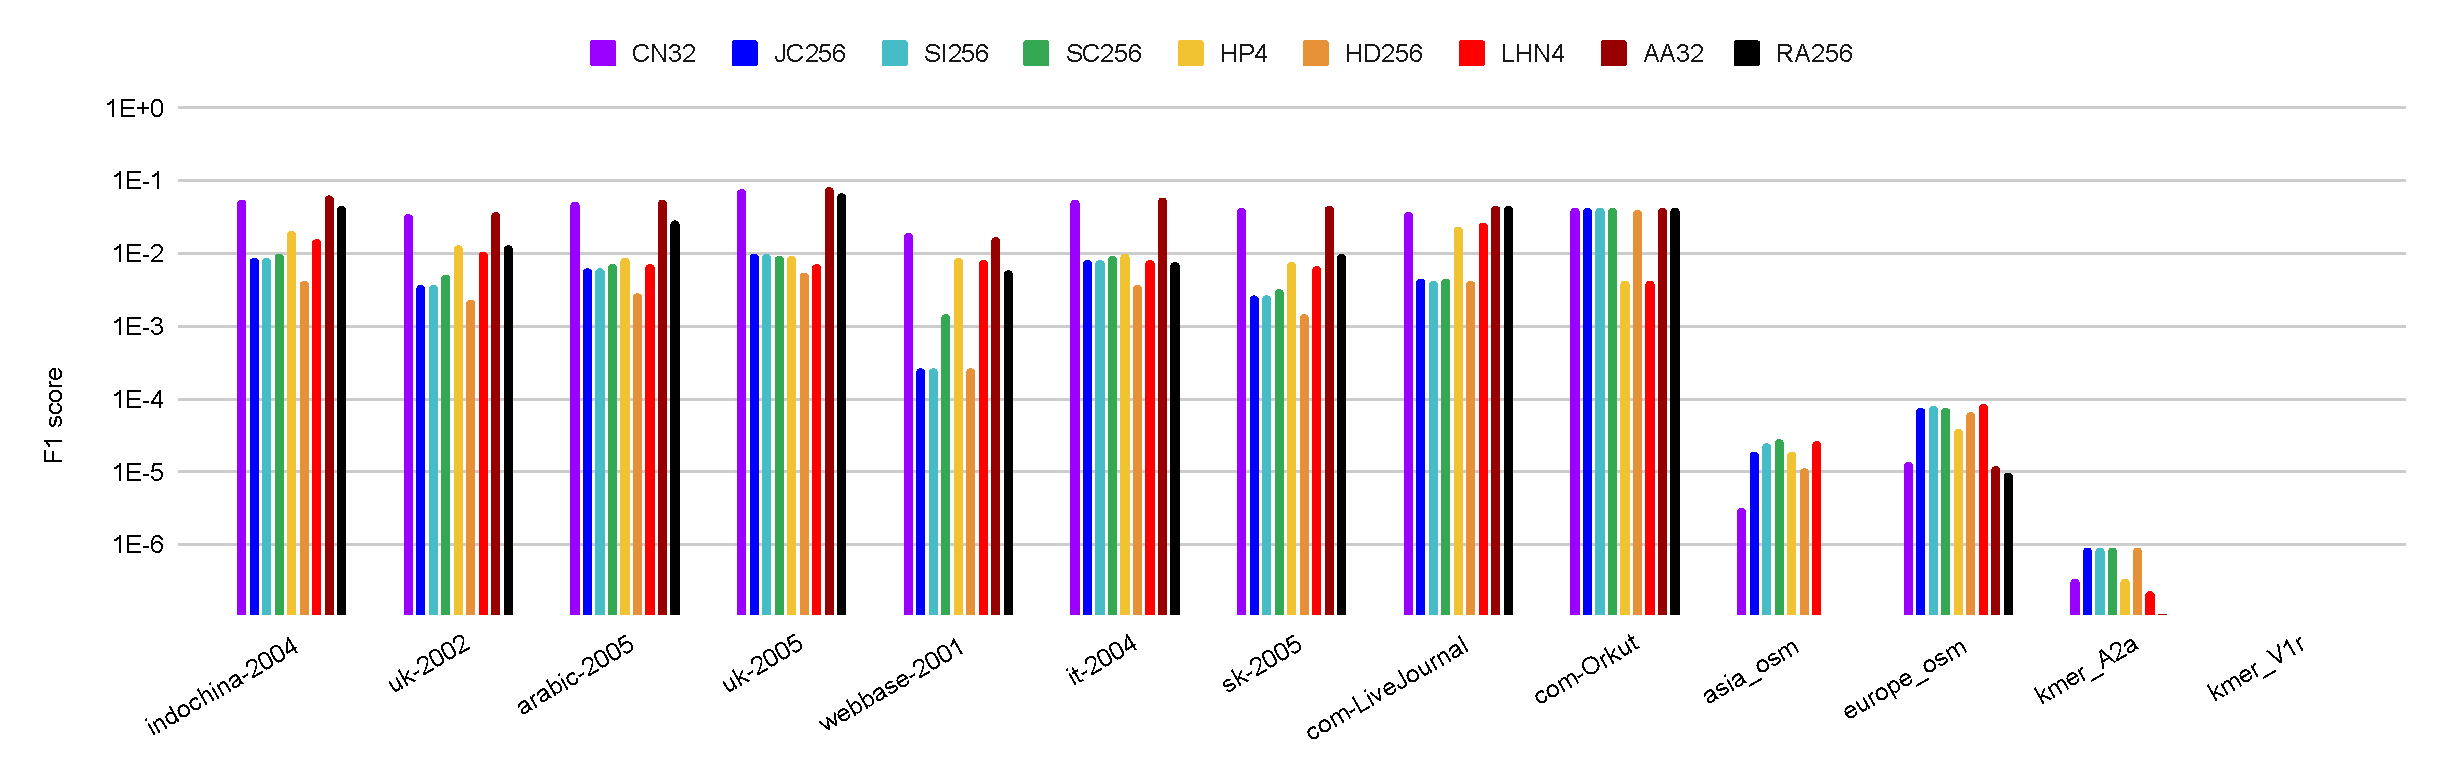
\includegraphics[width=0.98\linewidth]{out/pruned2-f1score.pdf}
  } \\[-2ex]
  \caption{TODO. Runtime in seconds (log-scale), and precision of predicted links, in percentage (log-scale), of the best neighborhood-based link prediction method (considering both the precision and runtime), on batch sizes of $10^{-4}|E|$ to $0.1|E|$ for each graph in the dataset. None of the methods succeed in predicting ground-truth links for \textit{kmer\_V1r}, and for \textit{asia\_osm} and \textit{kmer\_A2a} on batch sizes of $10^{-4}|E|$ to $10^{-3}|E|$, and thus their results are not shown. Note that the numerical suffix added to the acronym of each link prediction method indicates the hub limit $L_H$ parameter setting.}
  \label{fig:pruned2}
\end{figure*}

\begin{figure*}[hbtp]
  \centering
  \subfigure[Runtime in seconds (logarithmic scale) for link prediction using various similarity measures, with IHub approach]{
    \label{fig:pruned1--runtime}
    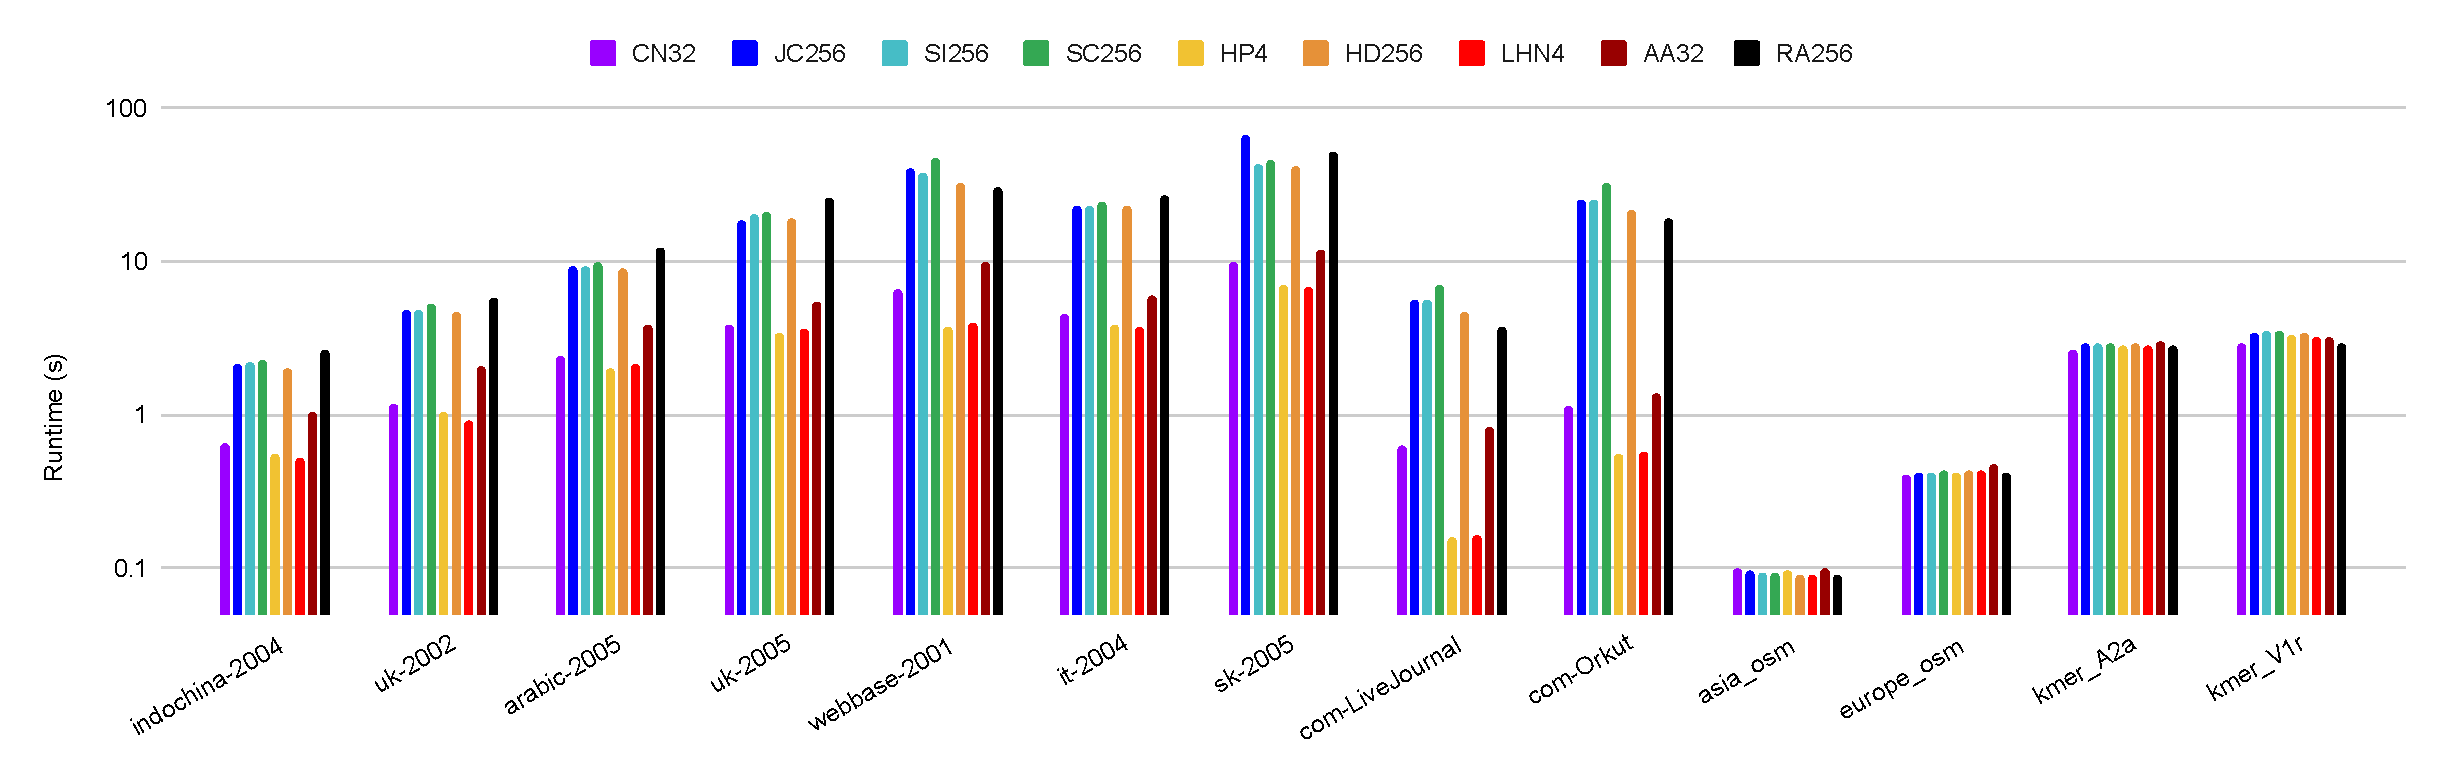
\includegraphics[width=0.98\linewidth]{out/pruned1-runtime.pdf}
  }
  \subfigure[Precision of predicted links, in percentage (logarithmic scale), of the best neighborhood-based link prediction method]{
    \label{fig:pruned1--f1score}
    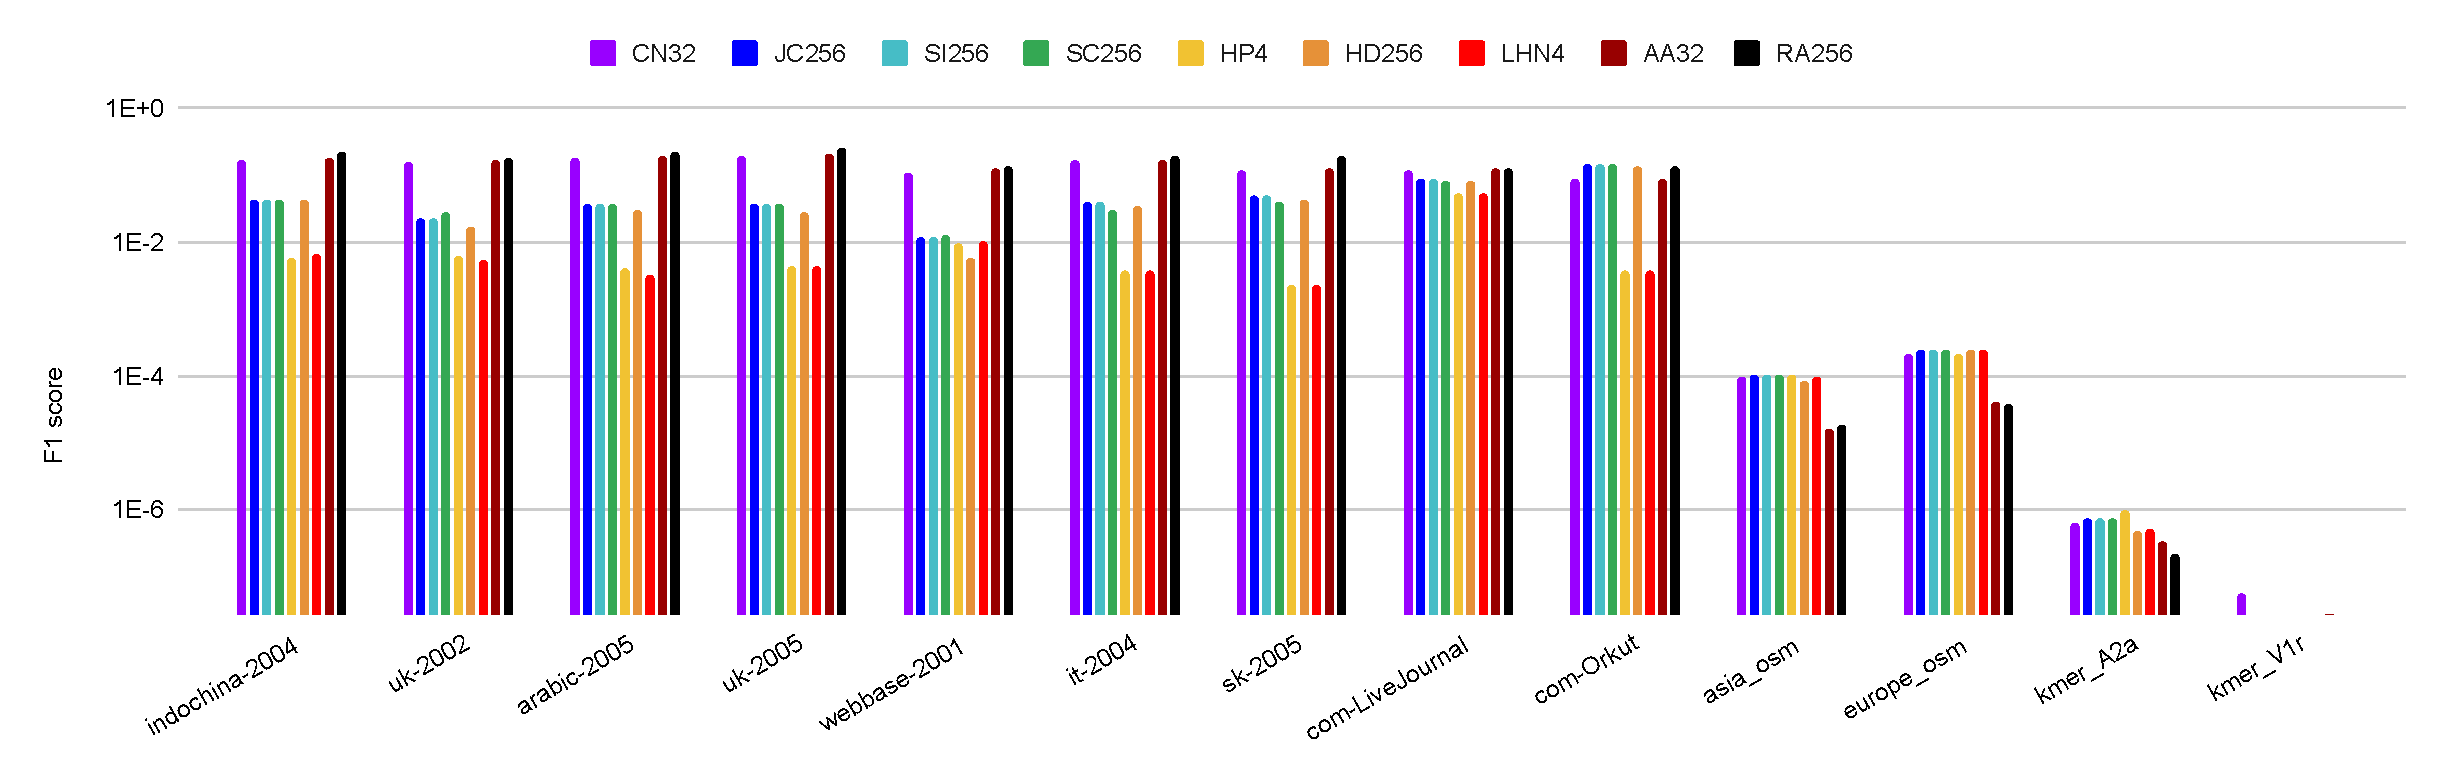
\includegraphics[width=0.98\linewidth]{out/pruned1-f1score.pdf}
  } \\[-2ex]
  \caption{TODO. Runtime in seconds (log-scale), and precision of predicted links, in percentage (log-scale), of the best neighborhood-based link prediction method (considering both the precision and runtime), on batch sizes of $10^{-4}|E|$ to $0.1|E|$ for each graph in the dataset. None of the methods succeed in predicting ground-truth links for \textit{kmer\_V1r}, and for \textit{asia\_osm} and \textit{kmer\_A2a} on batch sizes of $10^{-4}|E|$ to $10^{-3}|E|$, and thus their results are not shown. Note that the numerical suffix added to the acronym of each link prediction method indicates the hub limit $L_H$ parameter setting.}
  \label{fig:pruned1}
\end{figure*}


\end{document}
\endinput
%% End of file.




%% NOTES:
%% - Parallelization seems to be not efficient for small batch updates.
%% - Discuss about conflicting updates
%% - 


%% TODO:
%% - Scale up the size of the graphs
%% - Move experiments to a better server
%% - Include a weak- and strong- scalabiilty plot: run the expt from 2 to 128 threads
%% - overall space planning
%% - add a few lines on novelty of the paper.
%% - table comparison of related work
%% - Include a section on preliminaries that talks about the various algorithmic ideas (Louvain, Label Propagation)

%% Workplan:
%% - KK -- Read Introduction, Related Work,
%% - Dip Sankar -- Approach -- summarize the main algorithmic ideas,
%% - Subhajit -- Results -- Plots, scalability, Dataset, experiments, implementation details,
